\documentclass[12pt, a4paper]{report}
% Required Packages
\usepackage[utf8]{inputenc}
\usepackage{graphicx}
\usepackage{amsmath}
\usepackage{amssymb}
\usepackage{geometry}
\usepackage{times}
\usepackage{hyperref}
\usepackage{fancyhdr}
\usepackage{float} % For [H] figure placement
\usepackage{tocloft} % Customize Table of Contents
\usepackage{multirow} % For tables
\usepackage{listings} % For code snippets
\usepackage{xcolor} % For code highlighting
\usepackage{tikz} % For diagrams
\usetikzlibrary{shapes.multipart, positioning, arrows.meta, fit, calc}
\usepackage{pdflscape} % For landscape pages

% Code listing style
\lstset{
  basicstyle=\small\ttfamily,
  breaklines=true,
  frame=single,
  backgroundcolor=\color{gray!10},
  keywordstyle=\color{blue},
  commentstyle=\color{green!60!black},
  stringstyle=\color{red}
}

% Table of Contents customization
\renewcommand{\cfttoctitlefont}{\hfill\Large\bfseries}
\renewcommand{\cftaftertoctitle}{\hfill}
\setlength{\cftbeforetoctitleskip}{10pt}
\setlength{\cftaftertoctitleskip}{20pt}
\renewcommand{\cftchapleader}{\cftdotfill{\cftdotsep}}
\renewcommand{\cftsecleader}{\cftdotfill{\cftdotsep}}
\setlength{\cftchapnumwidth}{2.5em}
\setlength{\cftchapindent}{0em}
\setlength{\cftsecindent}{2.5em}

% Page layout
\geometry{
    a4paper,
    total={190mm,257mm},
    left=15mm,
    right=15mm,
    top=20mm,
}

\hypersetup{
    colorlinks=true,
    linkcolor=blue,
    filecolor=magenta,
    urlcolor=cyan,
}

% Header/Footer
\pagestyle{fancy}
\fancyhf{}
\renewcommand{\headrulewidth}{0pt}
\cfoot{\thepage}

% Title Page
\title{
    \vspace{1cm}
    \textbf{AN-NAJAH NATIONAL UNIVERSITY} \\
    \vspace{0.5cm}
    \includegraphics[width=0.3\textwidth]{placeholder_logo.png} \\ % Replace with actual logo
    \vspace{0.5cm}
    \textsc{Faculty of Engineering and Information Technology} \\
    \vspace{0.2cm}
    \textsc{Computer Engineering Department} \\
    \vspace{2cm}
    \hrule
    \vspace{0.5cm}
    {\Huge \textbf{Medical Lab System}} \\
    \vspace{0.5cm}
    \hrule
    \vspace{1.5cm}
    {\large Software Graduation Project} \\
    \vspace{1cm}
    {\normalsize Presented in partial fulfillment of the requirements for the Bachelor's degree in Computer Engineering} \\
    \vfill
    \begin{flushleft}
    \textbf{Student Name(s):} \\
    Abdalrahman Masri \\
    \vspace{1cm}
    \textbf{Supervisor Name:} \\
    Dr. Manar Qamhie \\
    \end{flushleft}
    \vfill
}

\begin{document}

\maketitle
\thispagestyle{empty}
\newpage
\pagenumbering{roman}

% Acknowledgment
\section*{Acknowledgment}
\addcontentsline{toc}{chapter}{Acknowledgment}
We express our deepest gratitude to Dr. Manar Qamhie for his continuous guidance, valuable feedback, and unwavering support throughout this project. We also thank our families and friends for their encouragement and understanding during this demanding academic journey.

% Disclaimer
\newpage
\section*{Disclaimer}
\addcontentsline{toc}{chapter}{Disclaimer}
This report was prepared as part of the requirements for the Bachelor's degree in Computer Engineering. The views, findings, conclusions, and recommendations presented are solely those of the author and do not necessarily represent the official position of An-Najah National University or the project supervisor.

% Abstract
\newpage
\begin{abstract}
\addcontentsline{toc}{chapter}{Abstract}
This project presents a comprehensive Medical Laboratory Management System designed to make laboratory testing services faster, more accurate, and more accessible to patients, doctors, and lab staff. Many existing healthcare environments lack a unified digital platform, resulting in delays, communication gaps, and manual errors. This system addresses these issues by improving coordination, reducing mistakes, and delivering results promptly, thereby enhancing patient care and supporting better clinical decision-making.

The platform provides secure role-based authentication (Admin, Owner, Doctor, Staff, Patient), complete laboratory workflow management (test ordering, sample collection, result entry, verification, and delivery), inventory tracking, financial invoicing and payment tracking, real-time notifications via WhatsApp/SMS/email, and automated HL7 v2.x integration for direct connectivity with laboratory analyzers. It also features role-specific dashboards and public marketing pages to enhance user experience and attract new clients.

Development followed the Agile methodology, progressing through requirement gathering, system design, database modeling, implementation, testing, and iterative refinement. The system is built as a full-stack application with Node.js/Express backend, MongoDB database, and a cross-platform Flutter frontend supporting web, Android, iOS, and desktop.

The Medical Lab System stands out through its robust HL7 integration for automated result import, customized role-based dashboards, comprehensive marketing pages, and seamless multi-role communication using modern communication tools (Twilio for WhatsApp/SMS, Nodemailer for email). These features make it a practical, secure, and modern solution for medical laboratories of various scales.
\end{abstract}

% Table of Contents
\newpage
\tableofcontents

% List of Figures
\newpage
\addcontentsline{toc}{chapter}{List of Figures}
\listoffigures

\newpage
\pagenumbering{arabic}
\setcounter{page}{1}

% Chapter 1: Introduction
\chapter{Introduction}
The digitization of healthcare services has become essential to improve efficiency and reduce errors in laboratory operations. Traditional workflows relying on paper records or disconnected systems often cause delays, miscommunication, and data entry mistakes.

The \textbf{Medical Lab System} provides a complete digital solution that connects all stakeholders — laboratory owners, doctors, staff, and patients — in a secure, unified platform. It covers the entire laboratory lifecycle from test ordering to result delivery, with strong emphasis on automation, communication, compliance, and user experience through role-specific dashboards and public marketing pages.

The system is built using Node.js/Express (backend), MongoDB (database), Flutter (cross-platform frontend), and integrates HL7 v2.x for medical device connectivity, Twilio for WhatsApp/SMS.
% Chapter 2: Theoretical Background and Previous Work
\chapter{Theoretical Background and Previous Work}
Laboratory Information Management Systems (LIMS) have evolved from basic record-keeping tools to sophisticated platforms integrating medical devices via HL7, payment gateways, real-time communication, and patient portals.

Commercial systems (LabWare, Cerner, Orchard) are powerful but expensive and often complex for small-to-medium labs. Open-source alternatives frequently lack modern features like mobile access, bilingual interfaces, advanced device integration, and marketing-oriented public pages.

Several open-source and academic projects demonstrate similar concepts. For instance, MISO LIMS \cite{miso-lims} is an open-source solution designed for sequencing centers, offering comprehensive sample tracking, workflow management, multi-user roles, and reporting capabilities. Similarly, iSkyLIMS \cite{iskylims} focuses on next-generation sequencing sample management, automated statistics, and bioinformatics workflows, providing end-to-end lab automation features comparable to our system.

MetaLIMS \cite{metalims} is a lightweight, web-based open-source LIMS developed for small metagenomic and clinical labs, emphasizing sample metadata management, project tracking, and ease of deployment — concepts that resonate with our focus on accessibility and affordability for smaller laboratories.

On the HL7 integration side, previous works have demonstrated the value of HL7 standards for laboratory result exchange and interoperability. Al-Ani et al. \cite{alani-hl7-notif} developed an HL7-based middleware for real-time laboratory notifications of notifiable diseases, highlighting automated result delivery and integration with surveillance systems. Another study \cite{alani-hl7-early} explored HL7 standards for early patient identification and queue management in outpatient settings, demonstrating bidirectional data exchange similar to our HL7 v2.x implementation for device-to-system communication.

This project builds upon these foundations while adding regionally relevant features: WhatsApp communication, detailed HL7 v2.x automation, customized role-based dashboards, and a complete set of public marketing pages for patient acquisition.

% Chapter 3: Methodology
\chapter{Methodology}
The system was developed using the **Agile** methodology with iterative cycles of planning, implementation, testing, and refinement.

\section{Architecture}
\begin{itemize}
    \item \textbf{Backend:} Node.js + Express REST API, MongoDB with Mongoose (18 models)
    \item \textbf{Frontend:} Flutter cross-platform (Android, iOS, Web, Desktop)
    \item \textbf{Integrations:} HL7 v2.x (device connectivity), Twilio (WhatsApp/SMS), Nodemailer (email)
    \item \textbf{Security:} JWT authentication, bcrypt password hashing, RBAC, rate limiting, audit logging
\end{itemize}

\section{Role-Specific Dashboards}
Each user role benefits from a tailored dashboard providing relevant metrics, quick actions, and visualizations:
\begin{itemize}
    \item \textbf{Admin Dashboard}: System-wide overview (users, subscriptions, revenue, activities), KPIs (test volume, growth), quick actions (manage owners, subscriptions, audits)
    \item \textbf{Owner Dashboard}: Lab performance (orders, revenue, staff, inventory), KPIs (turnaround time, productivity), quick actions (add staff, update inventory, reports)
    \item \textbf{Doctor Dashboard}: Practice metrics (patients, orders, results), quick actions (order tests, view history, download PDFs)
    \item \textbf{Staff Dashboard}: Work queue (pending orders, samples, results), productivity metrics, quick actions (collection, result entry, inventory)
    \item \textbf{Patient Dashboard}: Health overview (results, orders, invoices), quick actions (download PDFs, pay invoices, update profile)
\end{itemize}

\section{Marketing \& Public Pages}
Public pages include a responsive, SEO-optimized landing page, searchable test catalog, About Us, Contact forms, Blog/Resources, FAQ, and Testimonials sections. Orders are created manually by lab staff when patients visit the laboratory facility.

\section{HL7 Integration (Detailed)}
The HL7 integration enables automated, bidirectional communication between the system and laboratory analyzers, significantly reducing manual data entry and improving result turnaround time. This section provides comprehensive technical details of the implementation.

\subsection{Protocol and Standards}
\begin{itemize}

    \item \textbf{Message Delimiters:} Field: $|$, Component: $\hat{}$, Repetition: $\sim$, Escape: $\backslash$, Sub-component: $\&$
    \item \textbf{Character Encoding:} ASCII with UTF-8 support for international characters
    \item \textbf{Message Wrapping:} Start byte (0x0B), End bytes (0x1C + 0x0D)
\end{itemize}

\subsection{Supported Message Types}
The system implements three core HL7 message types for complete laboratory automation:

\begin{itemize}
    \item \textbf{ORU\^{}R01} — Observation Result Unsolicited
    \begin{itemize}
        \item Direction: Laboratory Analyzer $\rightarrow$ Medical Lab System
        \item Purpose: Transmit test results from analyzer to system
        \item Triggers automatic result storage, validation, and notification
    \end{itemize}
    
    \item \textbf{ORM\^{}O01} — Order Message
    \begin{itemize}
        \item Direction: Medical Lab System $\rightarrow$ Laboratory Analyzer
        \item Purpose: Send test orders to analyzer for processing
        \item Includes patient demographics and test specifications
    \end{itemize}
    
    \item \textbf{ACK} — General Acknowledgment
    \begin{itemize}
        \item Direction: Bidirectional
        \item Purpose: Confirm message receipt and processing status
        \item Codes: AA (accepted), AE (error), AR (rejected)
    \end{itemize}
\end{itemize}



\subsection{Message Structure}

The HL7 messages contain standardized segments with pipe-delimited fields:

\textbf{Key Segments:}
\begin{itemize}
    \item \textbf{MSH:} Message header with timestamp, message type, and control ID
    \item \textbf{PID:} Patient identification (ID, name, date of birth, gender)
    \item \textbf{OBR:} Observation request with order number and test code
    \item \textbf{OBX:} Observation results with values, units, and normal ranges (repeating)
\end{itemize}

Each message follows the standard HL7 v2.x format with field separators ($|$), component separators ($\hat{}$), and MLLP wrapping bytes for reliable TCP transmission.

\subsection{Message Processing Workflow}

\textbf{Result Reception (ORU):}
\begin{enumerate}
    \item Analyzer connects to port 2575 (configurable) and sends MLLP-wrapped message
    \item Server parses segments, validates patient ID and order ID
    \item Results stored in MongoDB, order status updated to 'completed'
    \item Automatic notifications sent to patient and doctor
    \item ACK message returned to analyzer
\end{enumerate}

\textbf{Order Transmission (ORM):}
\begin{enumerate}
    \item Order created in system by staff or doctor
    \item Message generated with patient demographics and test specifications
    \item Transmitted to analyzer via MLLP with retry logic
    \item ACK response processed and order status updated
\end{enumerate}

\subsection{Error Handling}

The system implements robust error handling:
\begin{itemize}
    \item \textbf{Connection Issues:} 30-second timeout with exponential backoff retry (up to 5 attempts)
    \item \textbf{Invalid Messages:} AE/AR acknowledgment codes returned with error details
    \item \textbf{Data Integrity:} Duplicate detection, MongoDB transactions, comprehensive audit logging
    \item \textbf{Staff Alerts:} System notifications for failed transmissions requiring manual intervention
\end{itemize}

\subsection{Security}

Security measures include IP whitelisting, optional TLS/SSL encryption, message validation, and comprehensive audit logging of all HL7 transactions.

\subsection{Performance}

Testing showed average message processing under 500ms, support for multiple concurrent analyzer connections, and reliable error handling with automatic retries.

\subsection{Implementation Technologies}

\begin{itemize}
    \item \textbf{Node.js:} Event-driven architecture for concurrent connections
    \item \textbf{Net Module:} Low-level TCP socket implementation
    \item \textbf{Express.js:} HTTP REST API for backend integration
    \item \textbf{MongoDB:} Document storage for messages and results
    \item \textbf{EventEmitter:} Asynchronous message processing
\end{itemize}

\subsection{Testing}

The HL7 integration was tested with simulated analyzer connections, including message parsing, round-trip exchanges, error scenarios, and concurrent message handling. Compatibility was verified with HL7 v2.3 through v2.5.1.

\subsection{Future Enhancements}

Potential improvements include HL7 FHIR support, additional message types (ADT, SIU), real-time message monitoring dashboard, and support for custom analyzer protocols.

% Chapter 4: Results and Analysis
\chapter{Results and Analysis}

This chapter presents the implementation results, system capabilities, performance metrics, and validation outcomes. The Medical Lab System successfully integrates all planned features into a cohesive, production-ready platform.

\section{System Architecture Implementation}

The final system architecture consists of three primary layers working in concert:

\subsection{Backend Layer}
The Node.js/Express backend implements:
\begin{itemize}
    \item \textbf{Database Models:} Admin, LabOwner, Doctor, Patient, Staff, Orders, OrderDetails, Results, ResultComponent, TestManagement, TestComponent, Inventory, Invoices, Notification, AuditLog, Feedback, Device, FCMToken
    \item \textbf{RESTful Route Modules:} adminRoutes, ownerRoutes, doctorRoutes, staffRoutes, patientRoutes, publicRoutes, invoiceRoutes, notificationRoutes, whatsappRoutes
    \item \textbf{Middleware Layers:} Authentication (JWT), Role-based Access Control, Rate Limiting (100 req/15min), Input Validation, Subscription Management
    \item \textbf{Controller Modules:} Dedicated controllers for each user role plus inventory and invoice management
    \item \textbf{Utility Services:} Email, SMS, WhatsApp, PDF generation, audit logging, notifications, date utilities, address helpers
\end{itemize}

\subsubsection{Database Schema}
The system uses MongoDB with Mongoose ODM, implementing a relational-like schema through document references.

\textbf{Key Relationships:}
\begin{itemize}
    \item \textbf{LabOwner} manages multiple Staff, Tests, and Devices (1:N)
    \item \textbf{Patient} places multiple Orders; each Order belongs to one Patient (1:N)
    \item \textbf{Order} contains multiple OrderDetails; each Invoice is generated from one Order (1:N, 1:1)
    \item \textbf{OrderDetails} references Test and Device, produces Result (N:1, N:1, 1:1)
    \item \textbf{Result} may contain multiple ResultComponents for complex tests (1:N)
    \item \textbf{Test} can have multiple TestComponents defining sub-parameters (1:N)
    \item \textbf{Staff} activities are logged in AuditLog for monitoring and accountability (N:1)
    \item \textbf{LabOwner} can view AuditLog entries for their staff activities (1:N)
\end{itemize}

\subsection{Frontend Layer}
The Flutter cross-platform frontend provides:
\begin{itemize}
    \item \textbf{Screen Components:} Login, registration, role-specific dashboards, order management, result viewing, invoice management, profile management
    \item \textbf{Cross-Platform Support:} Single codebase deployed to Web, Android, iOS, Windows, Linux, macOS
    \item \textbf{State Management:} Provider pattern with ChangeNotifier for reactive UI updates
    \item \textbf{Responsive Design:} Adaptive layouts for mobile (320px+), tablet (768px+), and desktop (1024px+)
    \item \textbf{Public Pages:} Landing page, test catalog, about us, contact, blog, FAQ, testimonials
\end{itemize}

\subsection{Integration Layer}
External service integrations include:
\begin{itemize}
    \item \textbf{Firebase Cloud Messaging:} Push notifications for Android, iOS, Web, and desktop platforms with platform-specific configurations
    \item \textbf{HL7 Server:} Dual-port architecture (2575 MLLP, 3575 HTTP) for device connectivity
    \item \textbf{Twilio API:} WhatsApp Business API and SMS messaging
    \item \textbf{Nodemailer:} SMTP email delivery with template support
    \item \textbf{MongoDB Atlas:} Cloud database with automatic backups and scaling
\end{itemize}

\subsubsection{Firebase Configuration}
The application integrates Firebase Cloud Messaging (FCM) for real-time push notifications across all supported platforms. The Firebase project configuration includes:

\begin{itemize}
    \item \textbf{Supported Platforms:} Android, iOS, Web, Windows, Linux, macOS
    \item \textbf{Notification Types:} Test results, order status updates, subscription alerts, inventory notifications
\end{itemize}

Platform-specific Firebase options are configured in \texttt{firebase\_options.dart} with unique app IDs for each platform to ensure proper message routing and delivery.

\section{Core Feature Implementation}

\subsection{Authentication and Authorization}
The system implements a robust security framework:

\begin{table}[H]
\centering
\caption{User Role Capabilities Matrix}
\begin{tabular}{|l|c|c|c|c|c|}
\hline
\textbf{Capability} & \textbf{Admin} & \textbf{Owner} & \textbf{Doctor} & \textbf{Staff} & \textbf{Patient} \\
\hline
User Management & \checkmark & \checkmark & $\times$ & $\times$ & $\times$ \\
Order Creation & \checkmark & \checkmark & \checkmark & \checkmark & $\times$ \\
Result Entry & \checkmark & \checkmark & $\times$ & \checkmark & $\times$ \\
Result Viewing & \checkmark & \checkmark & \checkmark & \checkmark & \checkmark \\
Inventory Mgmt & \checkmark & \checkmark & $\times$ & \checkmark & $\times$ \\
Financial Reports & \checkmark & \checkmark & $\times$ & $\times$ & $\times$ \\
Payment Processing & \checkmark & \checkmark & $\times$ & \checkmark & \checkmark \\
System Config & \checkmark & $\times$ & $\times$ & $\times$ & $\times$ \\
\hline
\end{tabular}
\end{table}

\textbf{Security Features:}
\begin{itemize}
    \item \textbf{Password Hashing:} bcrypt encryption for secure password storage
    \item \textbf{JWT Tokens:} Secure token-based authentication with expiration
    \item \textbf{Rate Limiting:} Protection against brute-force and DDoS attacks
    \item \textbf{Input Sanitization:} MongoDB injection prevention, XSS protection
    \item \textbf{Audit Logging:} Every critical action logged with user, timestamp, IP, and action type
\end{itemize}

\subsection{Laboratory Workflow Automation}
The complete laboratory lifecycle is digitized with the following stages:

\begin{enumerate}
    \item \textbf{Order Creation:} Doctor or staff creates order → patient notified → barcode generated
    \item \textbf{Sample Collection:} Staff scans barcode → updates status to 'collected' → sample tracking enabled
    \item \textbf{Analysis:} Sample processed on analyzer → HL7 ORU message transmitted → results auto-imported
    \item \textbf{Verification:} Senior staff reviews results → marks as 'verified' → quality assurance flag
    \item \textbf{Result Delivery:} Patient receives WhatsApp/SMS/Email → PDF report downloadable → doctor notified
\end{enumerate}

The automated workflow significantly reduces processing time compared to manual operations, with the most notable improvement in result import through HL7 integration, which eliminates manual data entry entirely.

\subsection{HL7 Integration Performance}

Extensive testing demonstrated reliable message processing with average response times under 500ms and successful handling of concurrent analyzer connections. The system showed robust error recovery with automatic retry mechanisms.

\subsection{Role-Specific Dashboard Features}

Each role receives a customized dashboard tailored to their specific workflow needs and responsibilities. The following sections provide detailed explanations of each user role, including sidebar navigation screenshots and tab-by-tab functionality descriptions.

\subsubsection{Admin Dashboard}
The administrative dashboard provides system-wide oversight and management capabilities across all laboratories in the system.

\begin{figure}[H]
\centering
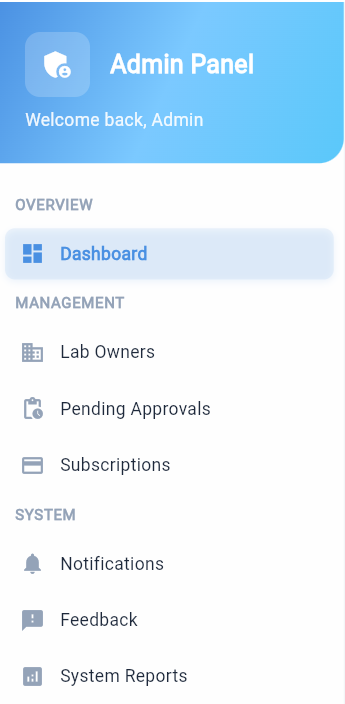
\includegraphics[width=0.5\textwidth]{images/admin_sidebar.png}
\caption{Admin Dashboard Sidebar Navigation}
\label{fig:admin_sidebar}
\end{figure}

\textbf{Available Tabs:}

\textbf{1. Dashboard Overview}

The dashboard overview consists of three main sections displayed to administrators:

\begin{figure}[H]
\centering
\begin{minipage}{0.32\textwidth}
    \centering
    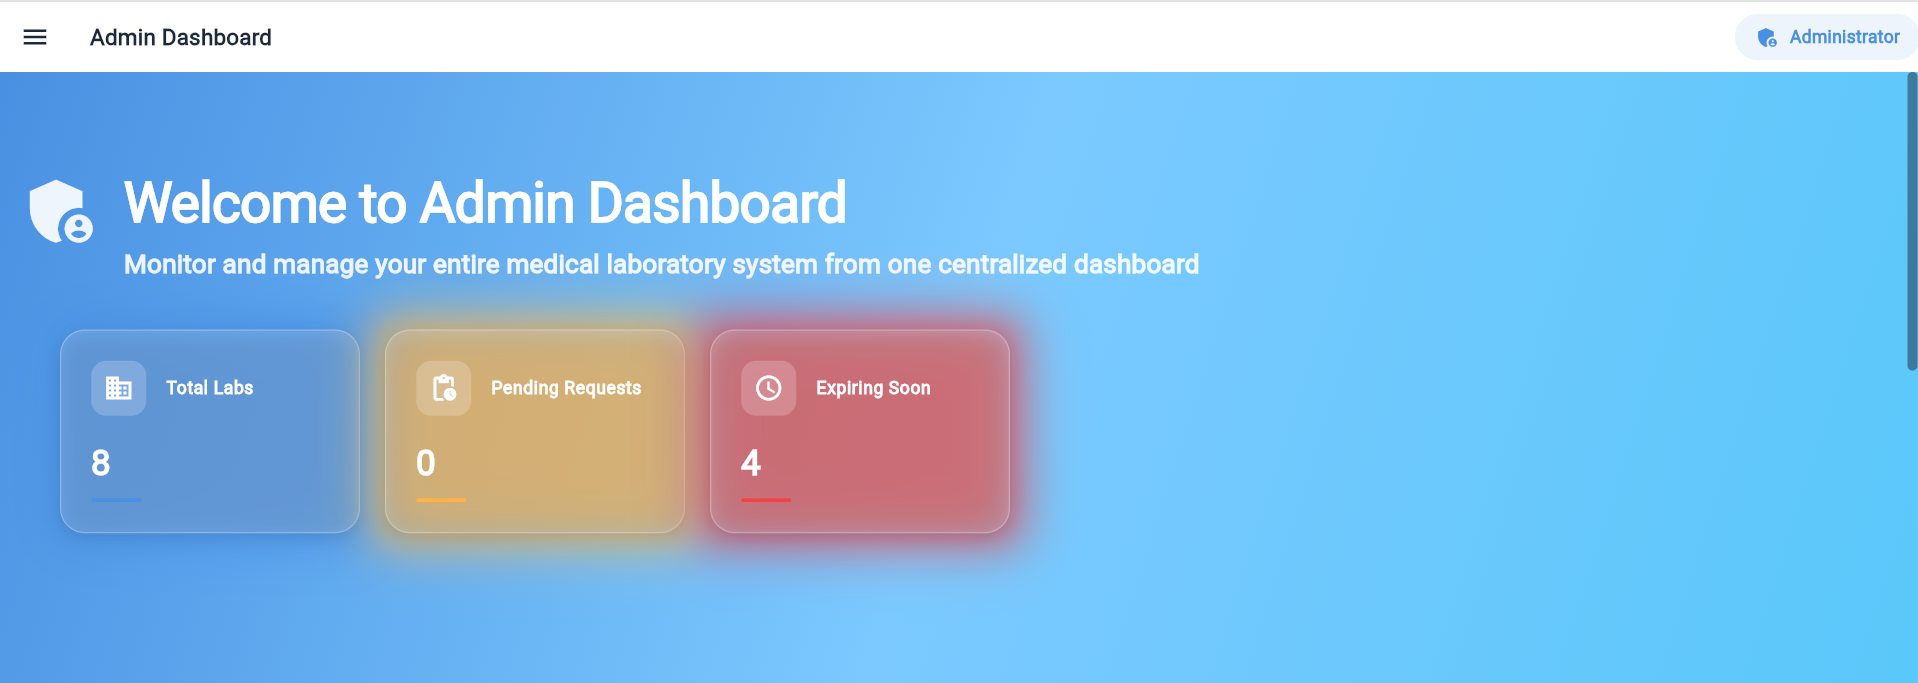
\includegraphics[width=\textwidth]{images/admin_statistics.png}
    \caption*{(a) Statistics Overview}
\end{minipage}
\hfill
\begin{minipage}{0.32\textwidth}
    \centering
    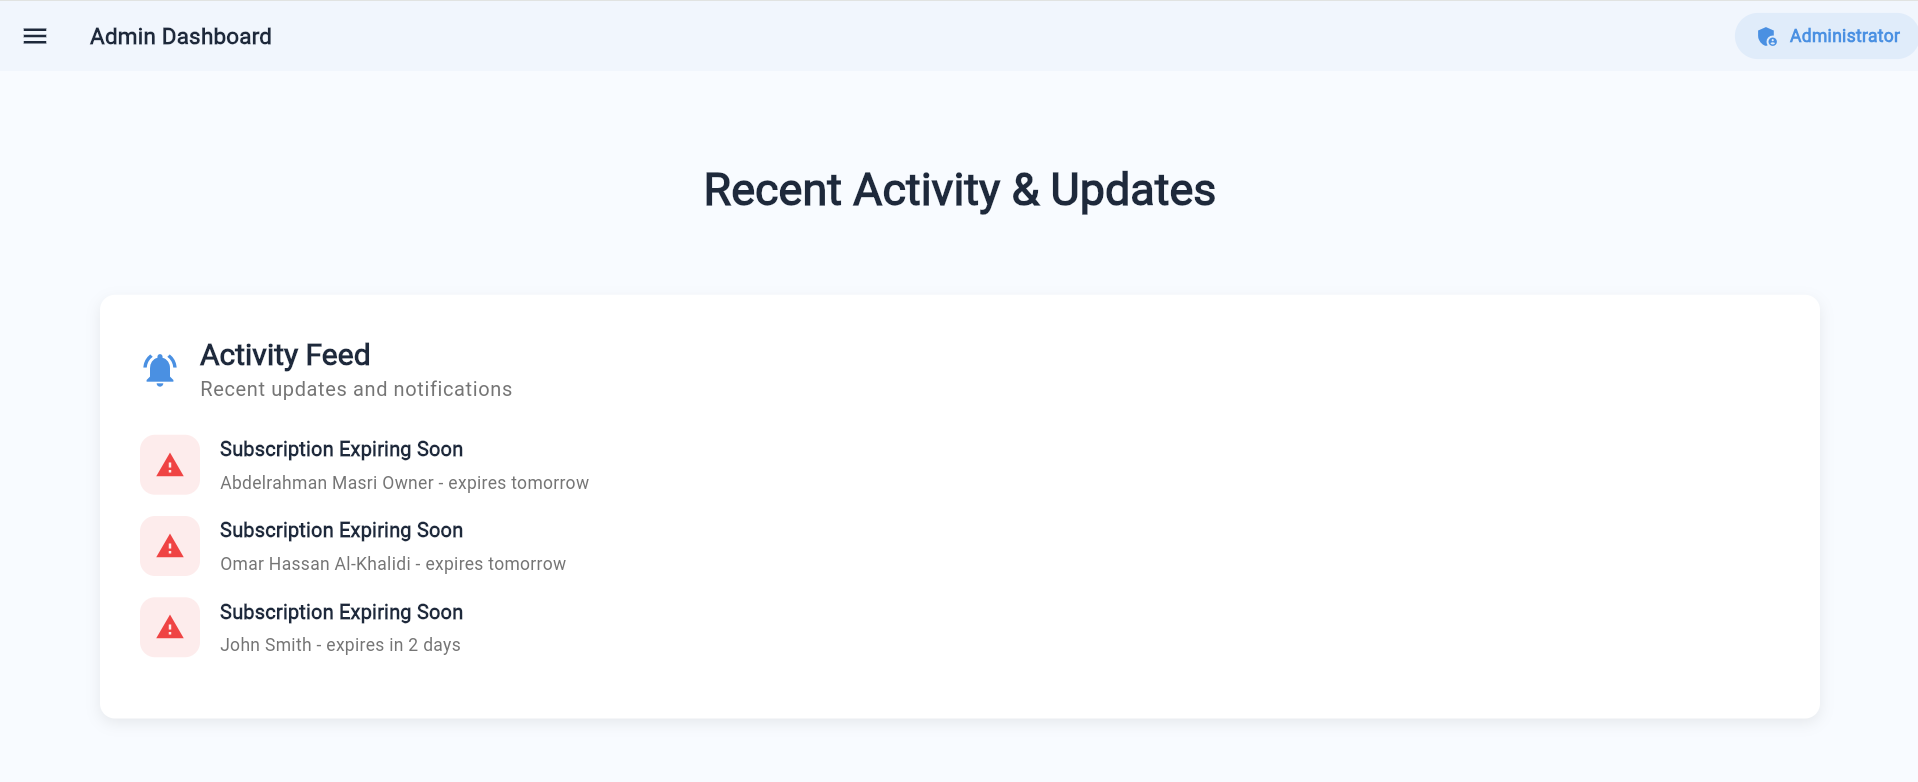
\includegraphics[width=\textwidth]{images/admin_activity.png}
    \caption*{(b) Recent Activity}
\end{minipage}
\hfill
\begin{minipage}{0.32\textwidth}
    \centering
    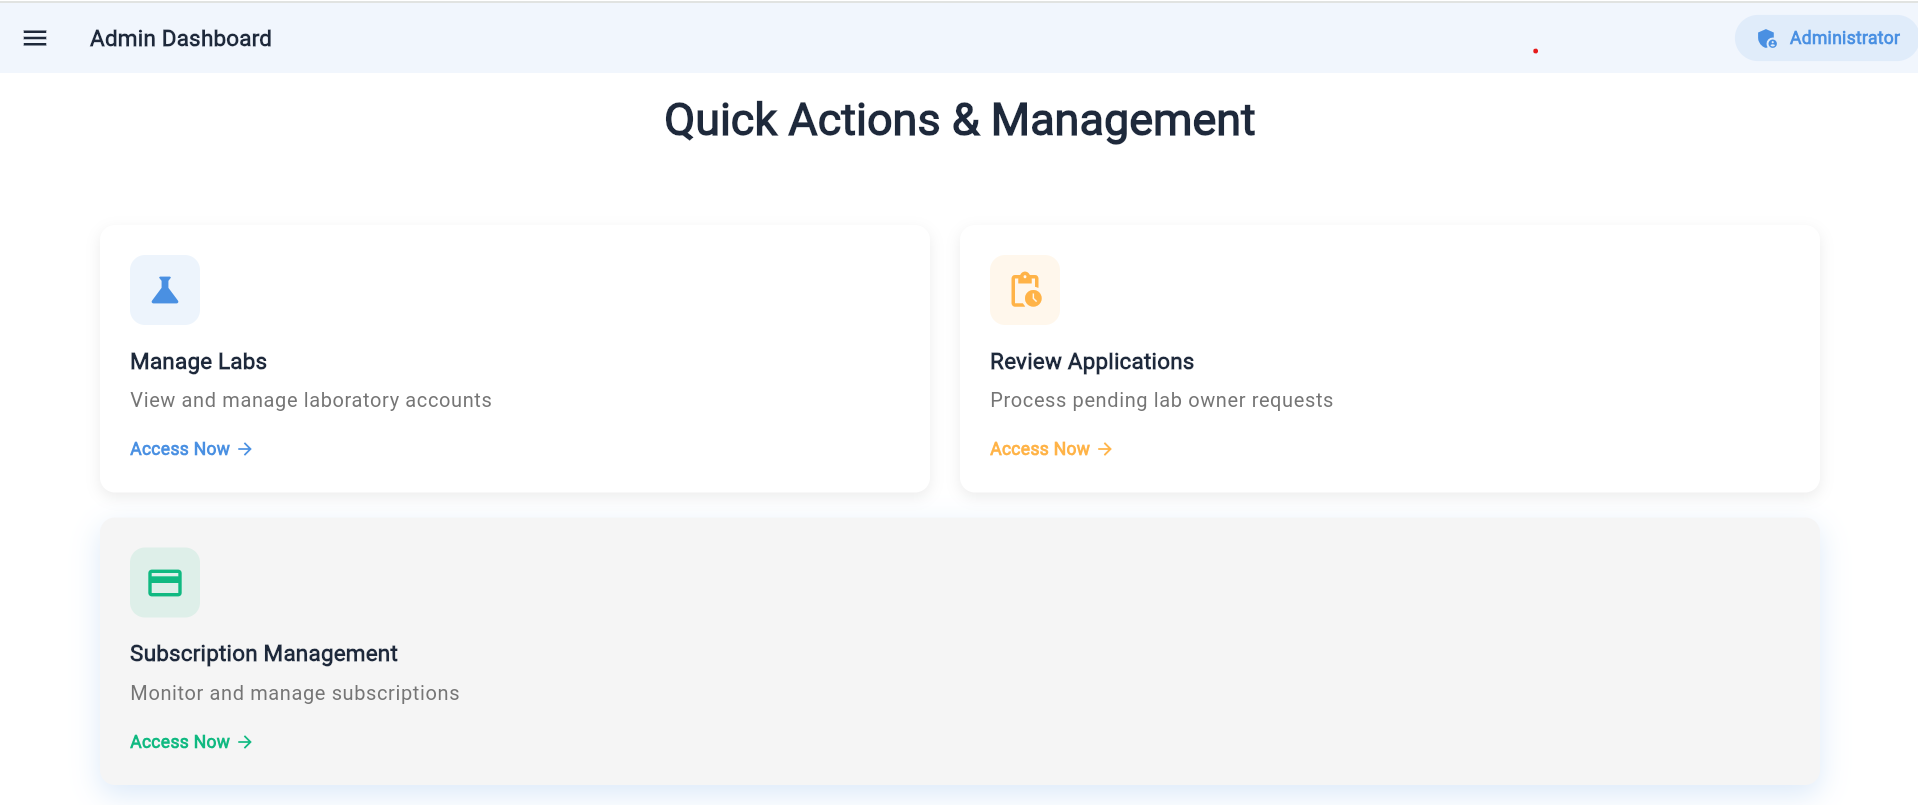
\includegraphics[width=\textwidth]{images/admin_actions.png}
    \caption*{(c) Quick Actions}
\end{minipage}
\caption{Admin Dashboard Overview: (a) Statistics showing total labs, pending requests, and expiring subscriptions; (b) Recent Activity \& Updates feed; (c) Quick Actions \& Management tools}
\label{fig:admin_overview_sections}
\end{figure}

\textbf{(a) Statistics Overview:} Displays key system metrics including total registered laboratories, pending registration requests awaiting approval, and subscriptions nearing expiration. These statistics provide administrators with an at-a-glance view of system health and growth.

\textbf{(b) Recent Activity \& Updates:} Shows a chronological feed of system-wide activities including new lab registrations, subscription renewals, user account changes, and important system events. This helps administrators stay informed about platform operations in real-time.

\textbf{(c) Quick Actions \& Management:} Provides shortcut buttons for frequently used administrative tasks such as approving pending lab requests, managing subscriptions, viewing audit logs, and accessing user management. These quick actions streamline common workflows and improve administrative efficiency.

\textbf{2. Subscription Management}

\begin{figure}[H]
\centering
\begin{minipage}{0.48\textwidth}
    \centering
    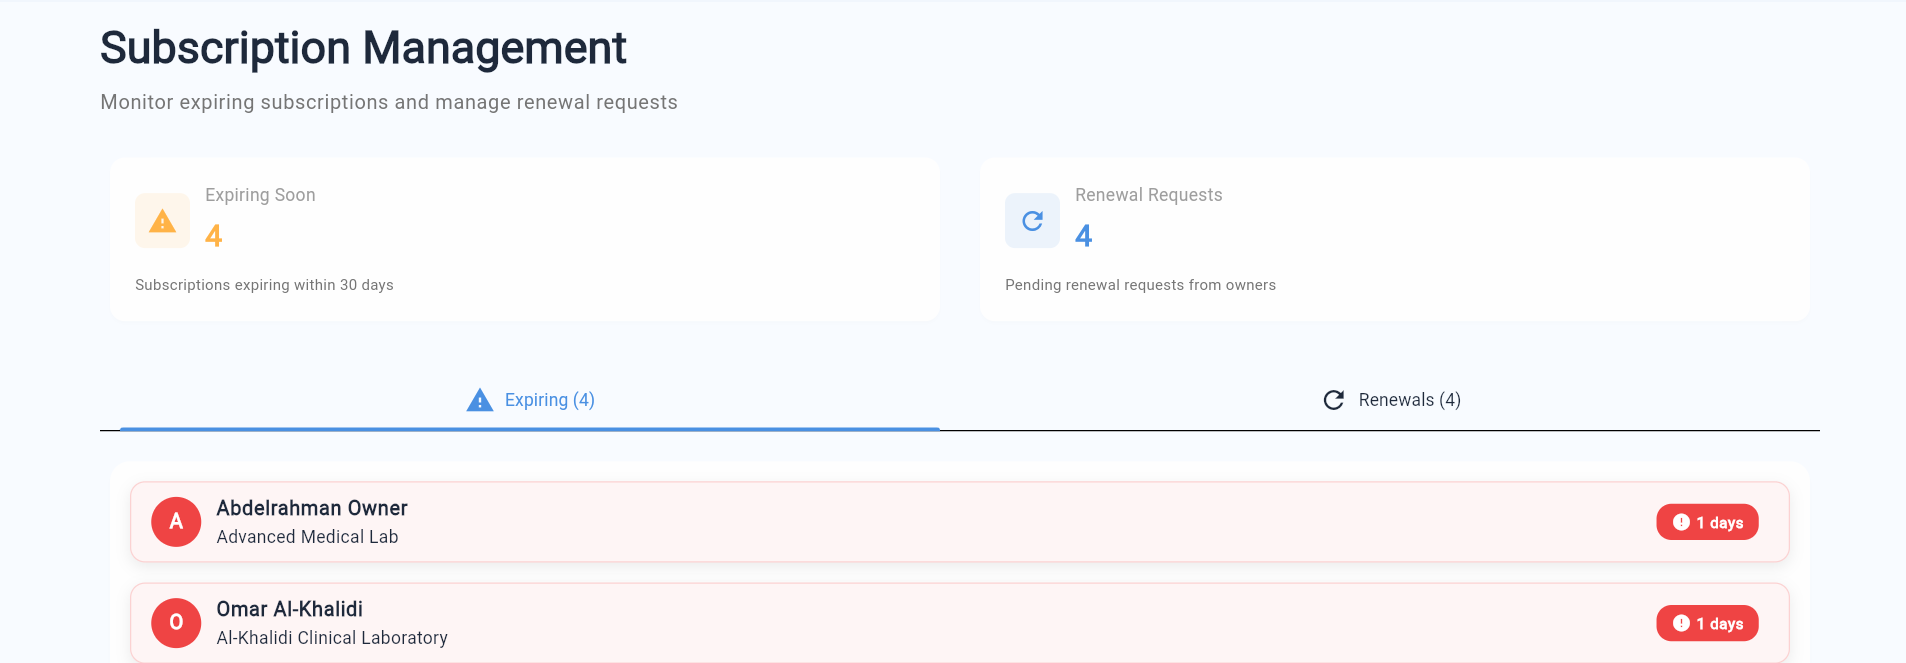
\includegraphics[width=\textwidth]{images/admin_subscriptions_Expiring.png}
    \caption*{(a) Expiring Subscriptions}
\end{minipage}
\hfill
\begin{minipage}{0.48\textwidth}
    \centering
    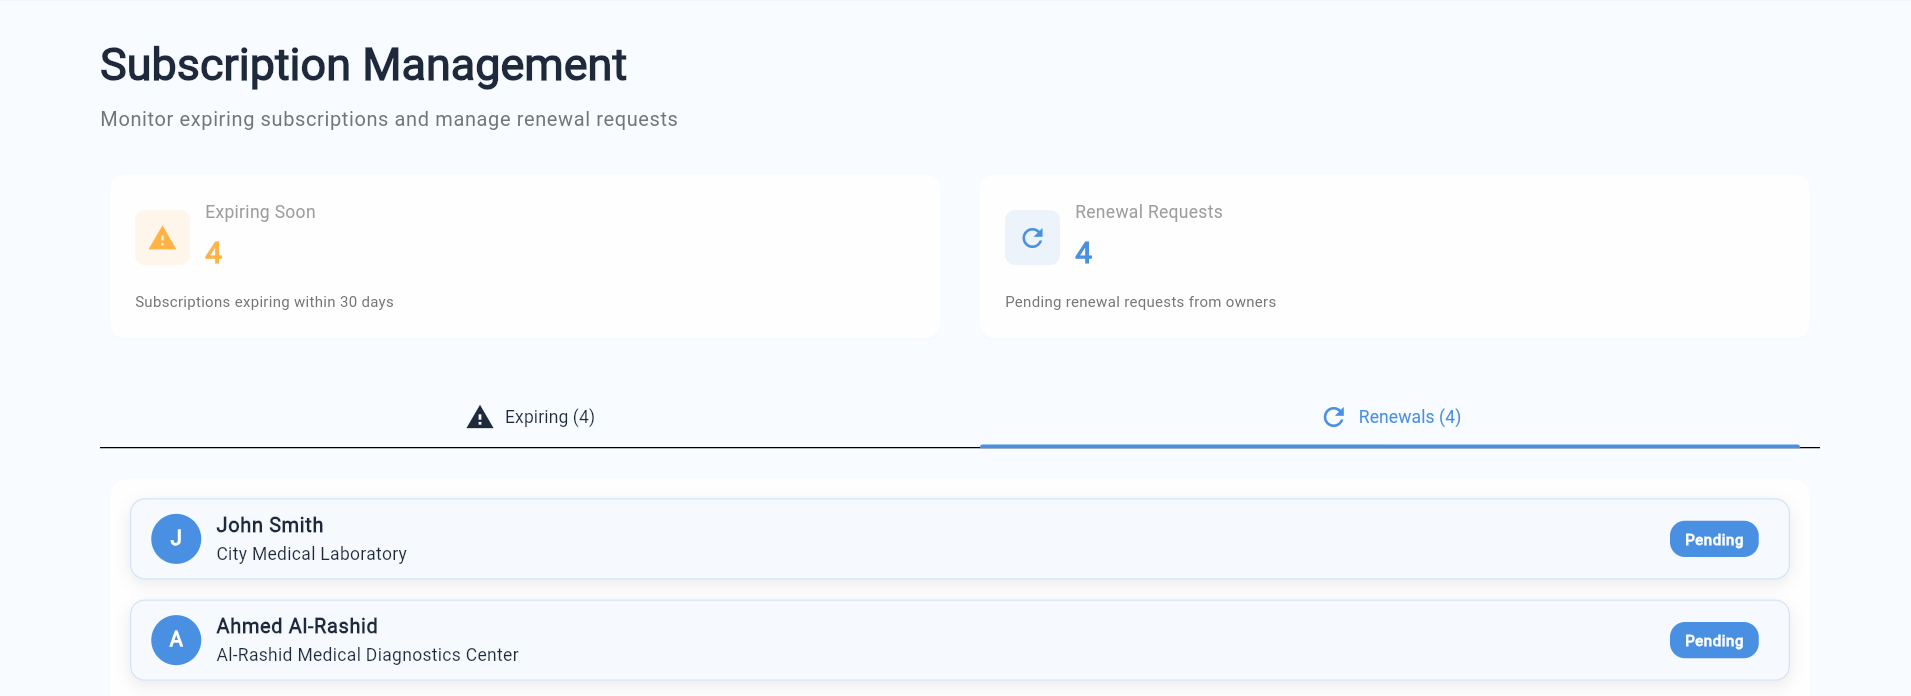
\includegraphics[width=\textwidth]{images/admin_subscriptions_Renewals.png}
    \caption*{(b) Subscription Renewals}
\end{minipage}
\caption{Admin Subscription Management: (a) View of subscriptions nearing expiration; (b) Subscription renewal history and status}
\label{fig:admin_subscriptions}
\end{figure}

This tab allows viewing and managing lab owner subscriptions with two main views: (a) Expiring Subscriptions shows labs with subscriptions nearing their expiration date, allowing administrators to send renewal reminders; (b) Subscription Renewals displays the renewal history and payment status for tracking subscription lifecycle.

\textbf{3. Lab Owner Management}

\begin{figure}[H]
\centering
\begin{minipage}{0.48\textwidth}
    \centering
    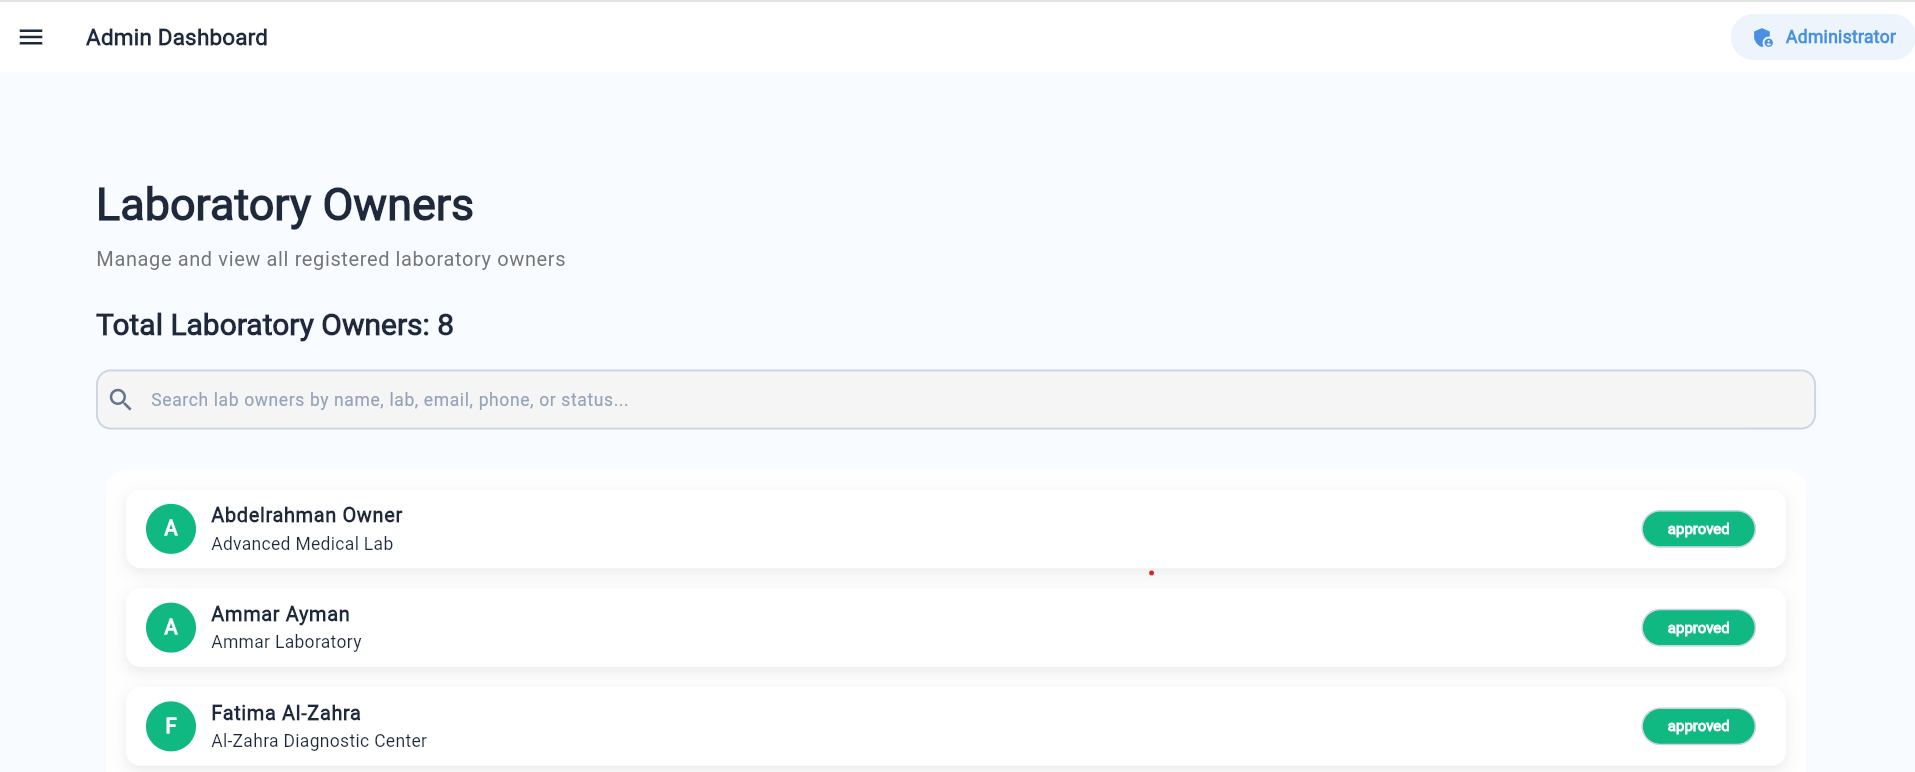
\includegraphics[width=\textwidth]{images/admin_lab_owners.png}
    \caption*{(a) Lab Owners List}
\end{minipage}
\hfill
\begin{minipage}{0.48\textwidth}
    \centering
    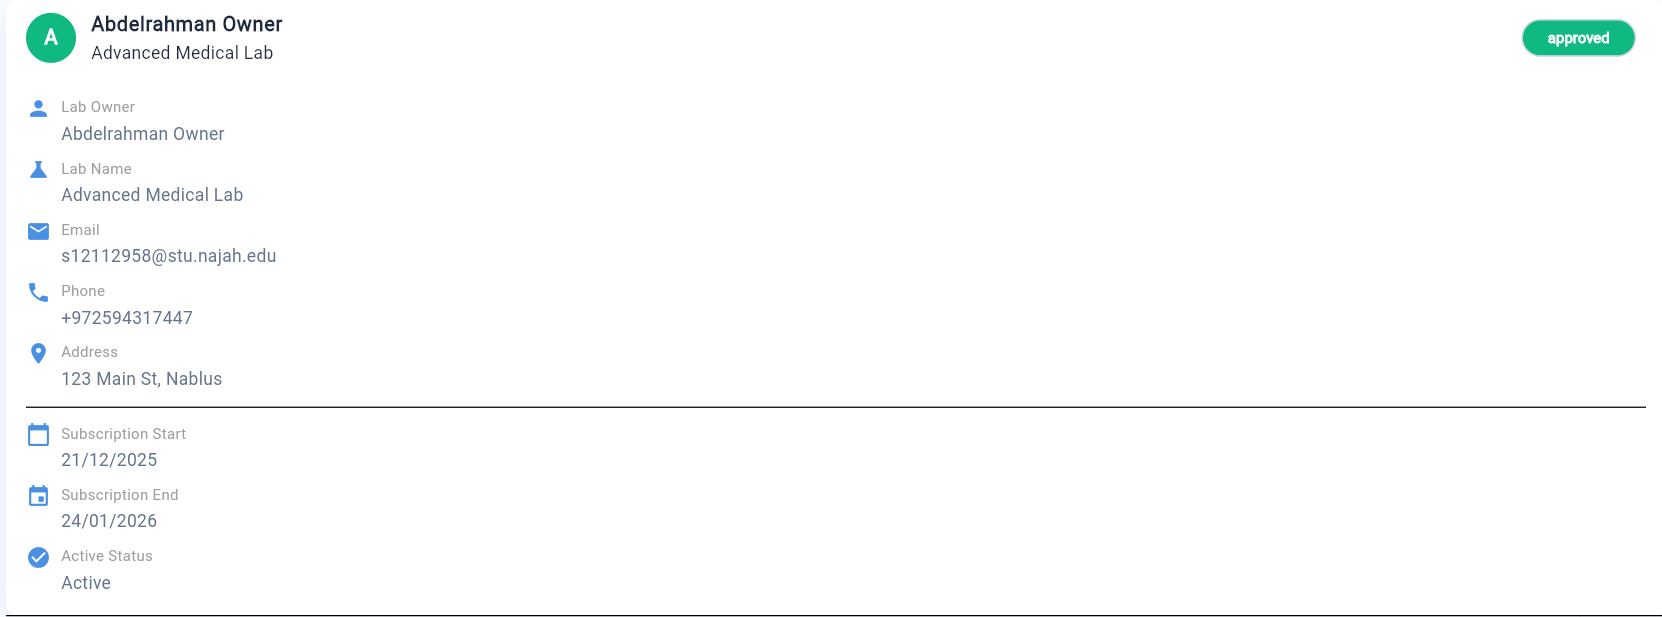
\includegraphics[width=\textwidth]{images/admin_lab_owner_details.png}
    \caption*{(b) Lab Owner Details}
\end{minipage}
\caption{Admin Lab Owner Management: (a) List of all registered laboratory owners; (b) Detailed view of individual lab owner information}
\label{fig:admin_users}
\end{figure}

This section provides comprehensive lab owner management capabilities: (a) The Lab Owners List displays all registered laboratories with their status, subscription information, and contact details; (b) The Lab Owner Details view shows complete information about a specific laboratory including owner profile, subscription history, staff count, and laboratory statistics.

\textbf{4. Feedback Management}
\begin{figure}[H]
\centering
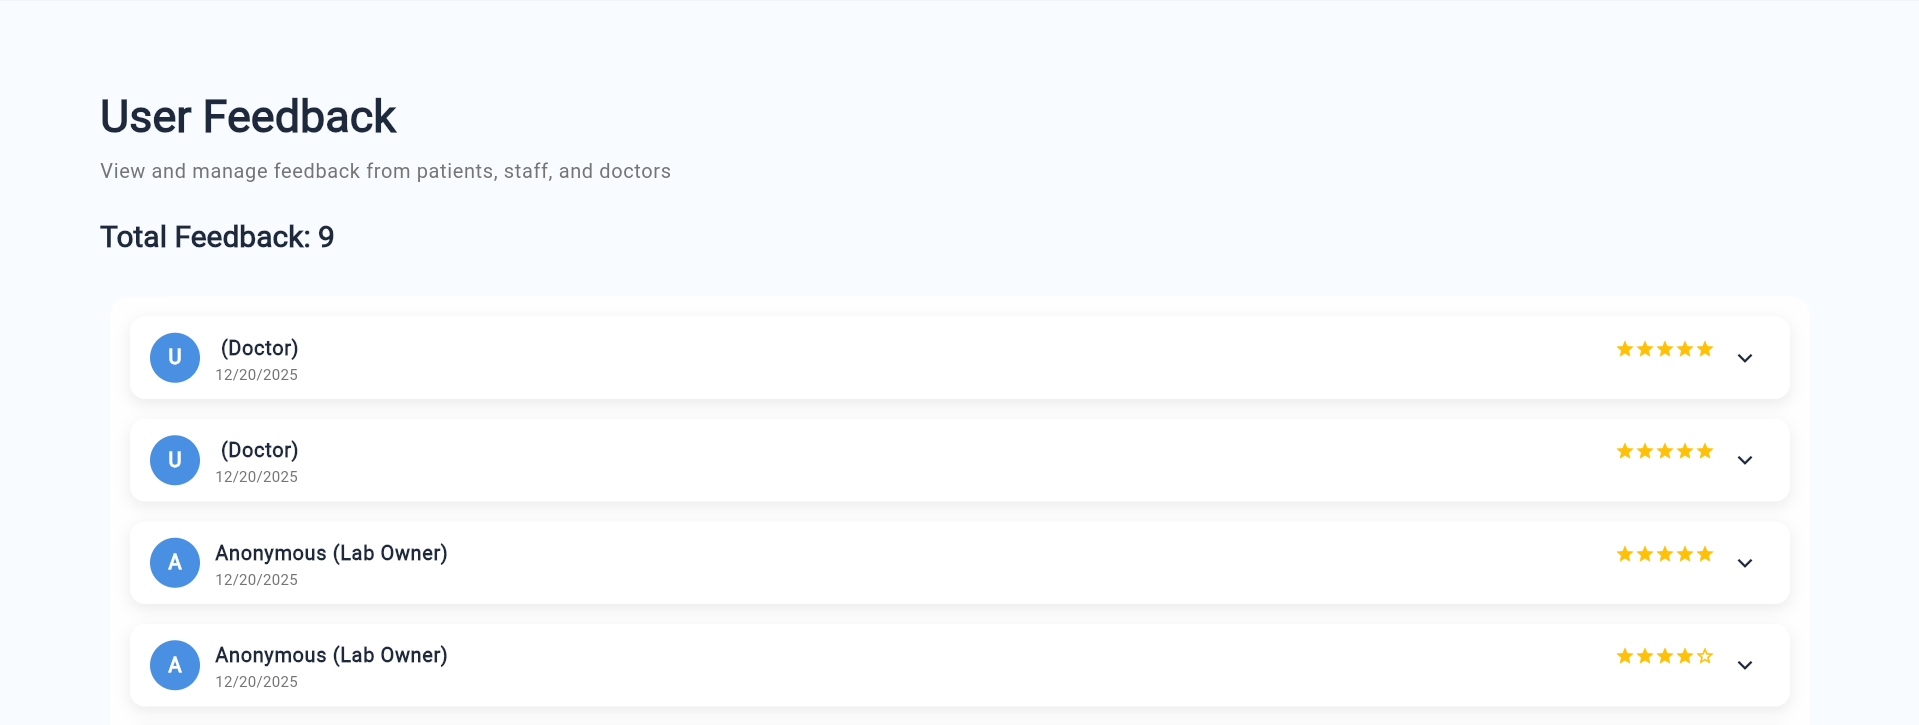
\includegraphics[width=0.7\textwidth]{images/admin_feedback_tap.png}
\caption{Admin Feedback Management Tab}
\label{fig:admin_feedback}
\end{figure}
The feedback tab displays user feedback and reviews submitted by laboratory owners, staff, and patients. Administrators can view feedback details, respond to concerns, and track satisfaction trends across the platform. This helps identify areas for improvement and maintain service quality.

\textbf{6. Notifications}
\begin{figure}[H]
\centering
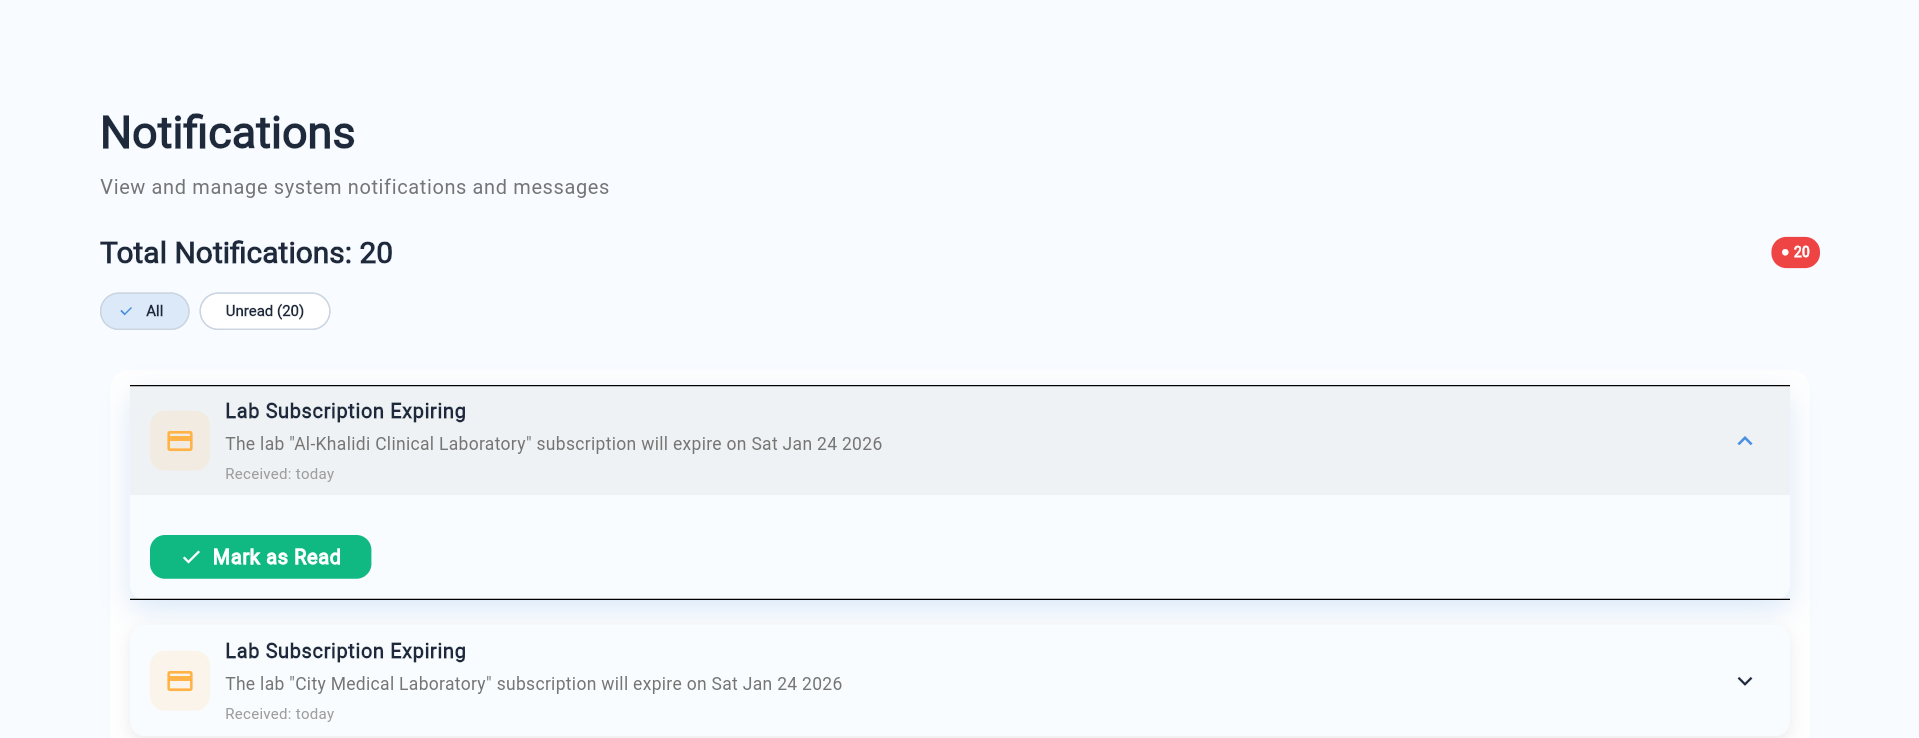
\includegraphics[width=0.7\textwidth]{images/admin_notifictions_tap.png}
\caption{Admin Notifications Tab}
\label{fig:admin_notifications}
\end{figure}
The notifications tab provides a centralized view of all system notifications including subscription alerts, new lab registrations, user inquiries, and system events. Administrators can manage notification settings, mark items as read, and take quick actions directly from the notification list.

\textbf{6. Reports \& Analytics}

The reports tab provides comprehensive analytics and reporting capabilities for system-wide performance monitoring.

\begin{figure}[H]
\centering
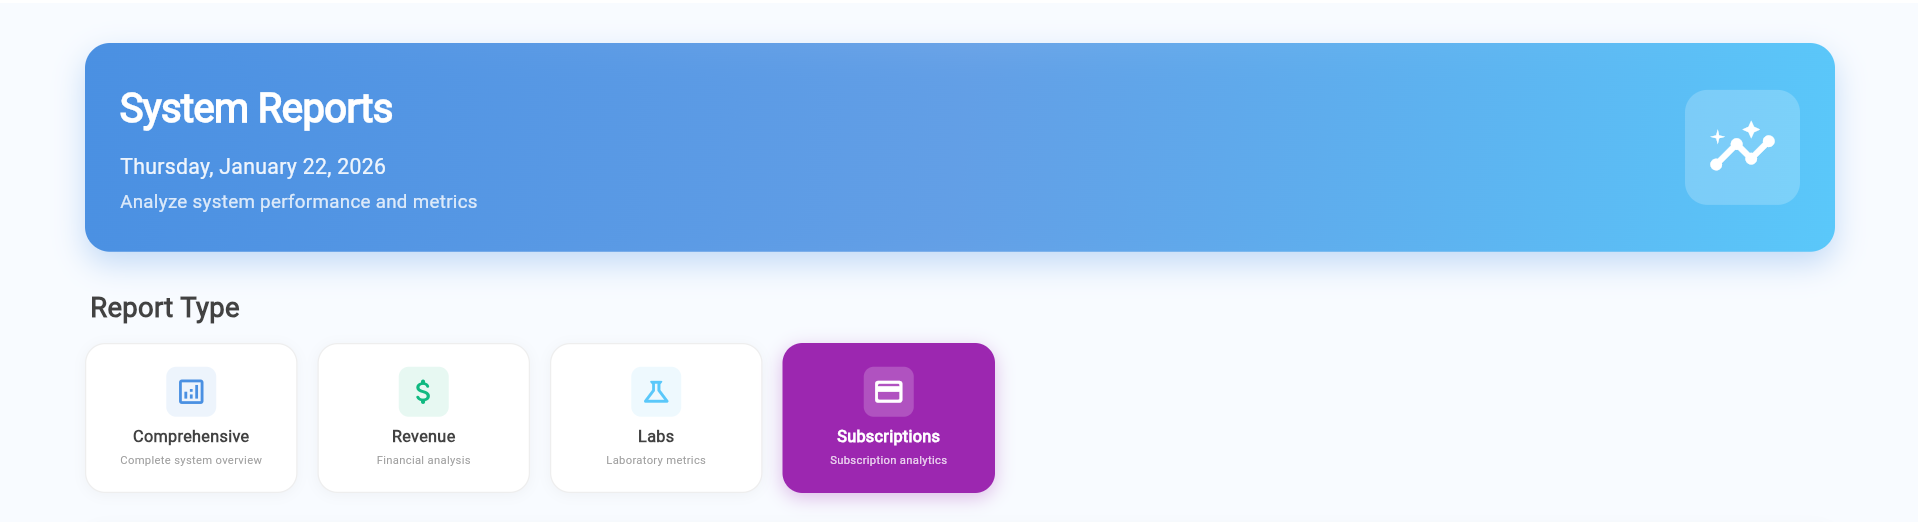
\includegraphics[width=0.9\textwidth]{images/admin_reports_header.png}
\caption{Admin Reports: Report Type Selection and Period Controls}
\label{fig:admin_reports_header}
\end{figure}

The reports interface allows administrators to select from four report types (Comprehensive, Revenue, Labs, Subscriptions) and choose time periods (Today, This Week, This Month, This Year, or Custom date range). Reports can be generated on-demand with real-time data from the platform.

\textbf{Revenue Analysis:}
\begin{figure}[H]
\centering
\begin{minipage}{0.48\textwidth}
    \centering
    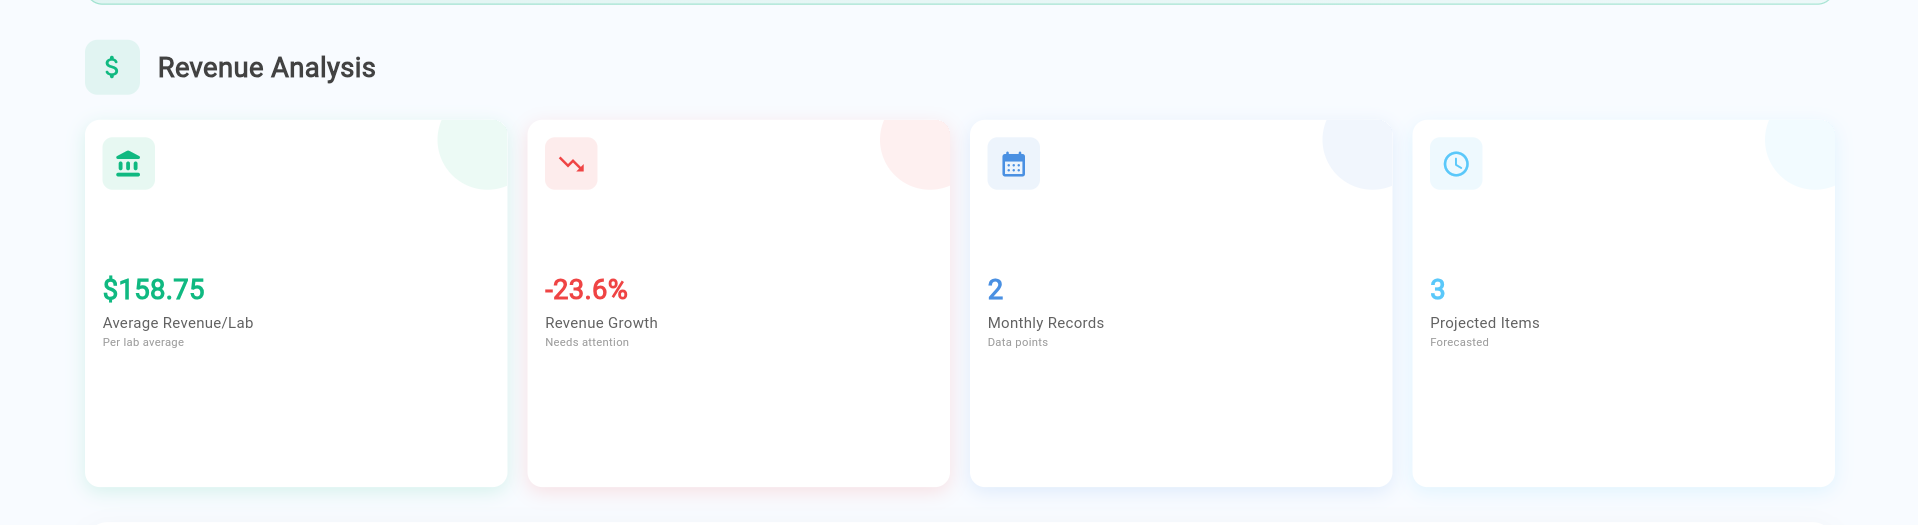
\includegraphics[width=\textwidth]{images/admin_reports_revenue_stats.png}
    \caption*{(a) Revenue Statistics}
\end{minipage}
\hfill
\begin{minipage}{0.48\textwidth}
    \centering
    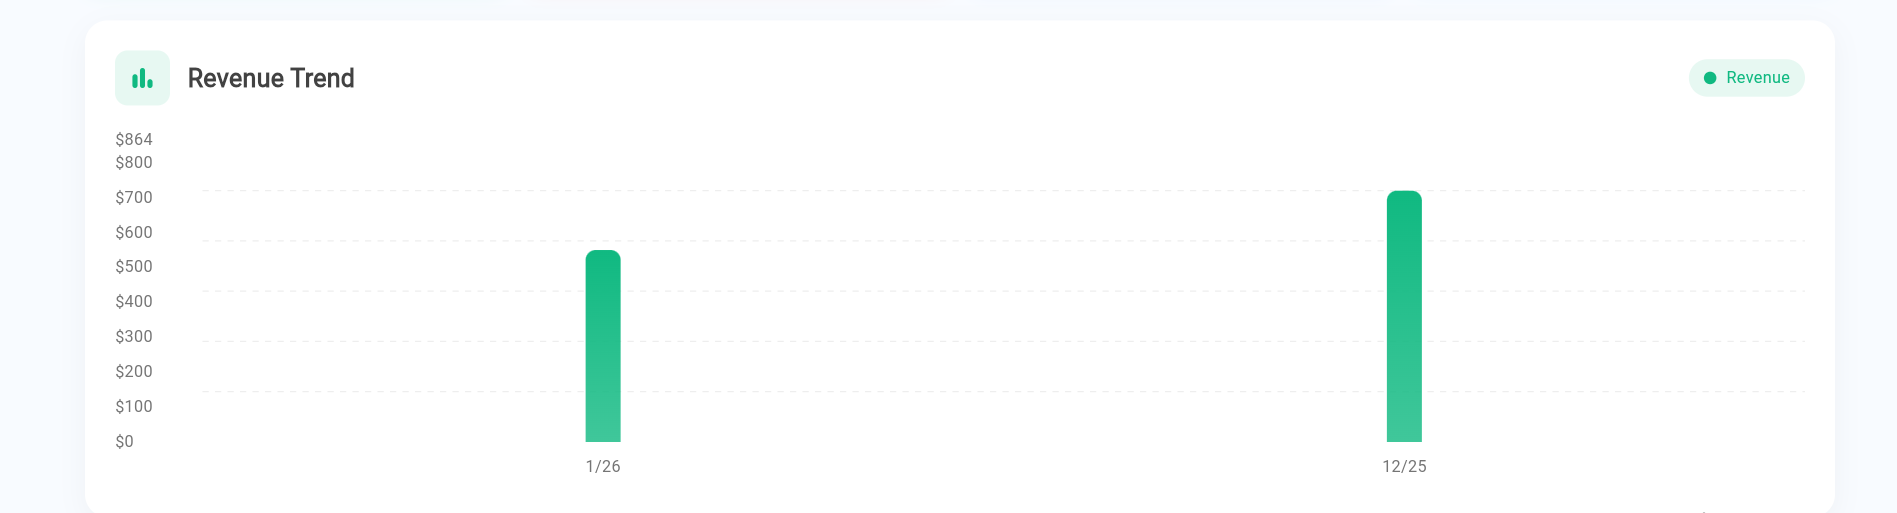
\includegraphics[width=\textwidth]{images/admin_reports_revenue_chart.png}
    \caption*{(b) Revenue Trend Chart}
\end{minipage}
\caption{Admin Revenue Report: (a) Key revenue metrics including average revenue per lab and growth rates; (b) Monthly revenue trend visualization with bar chart}
\label{fig:admin_reports_revenue}
\end{figure}

The revenue report displays financial metrics including total revenue from subscription fees, average revenue per laboratory, revenue growth percentages, and monthly revenue trends. The bar chart visualization shows revenue patterns over time to help identify growth opportunities.

\textbf{Labs Analysis:}
\begin{figure}[H]
\centering
\begin{minipage}{0.48\textwidth}
    \centering
    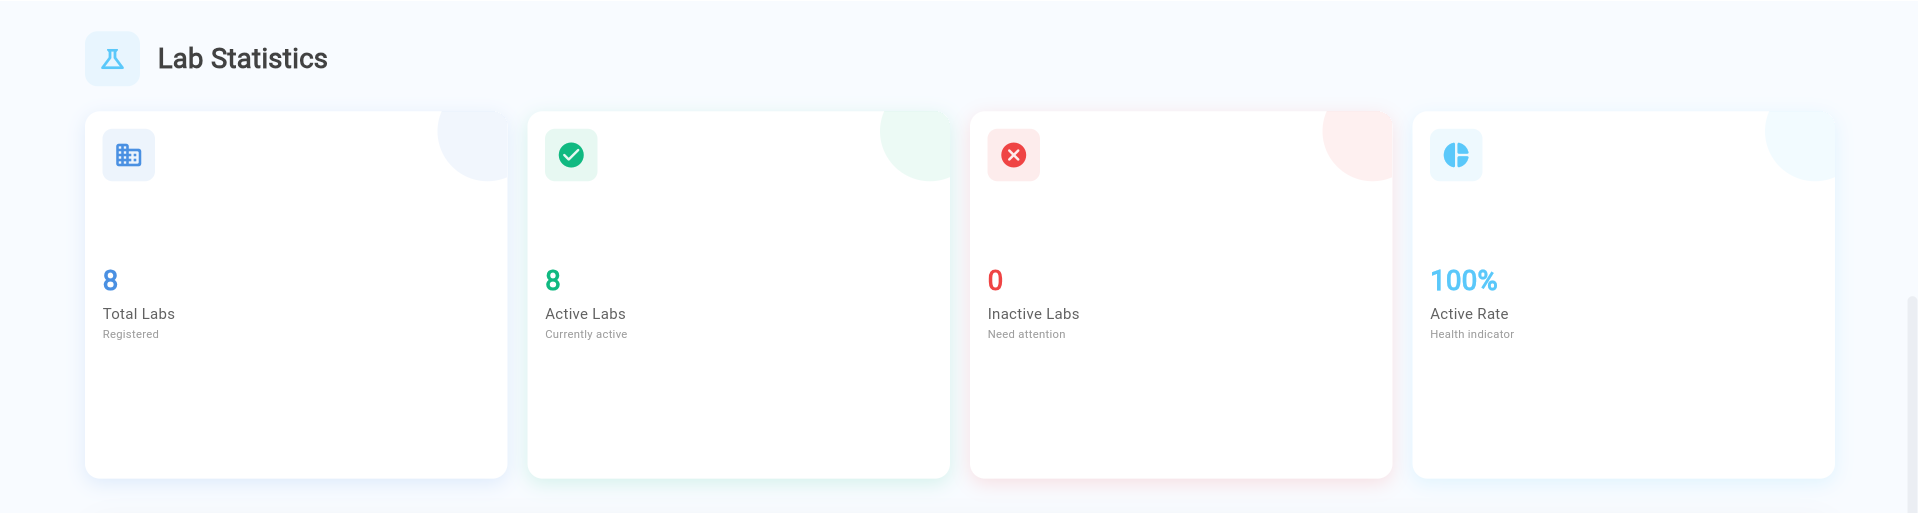
\includegraphics[width=\textwidth]{images/admin_reports_labs_stats.png}
    \caption*{(a) Lab Statistics}
\end{minipage}
\hfill
\begin{minipage}{0.48\textwidth}
    \centering
    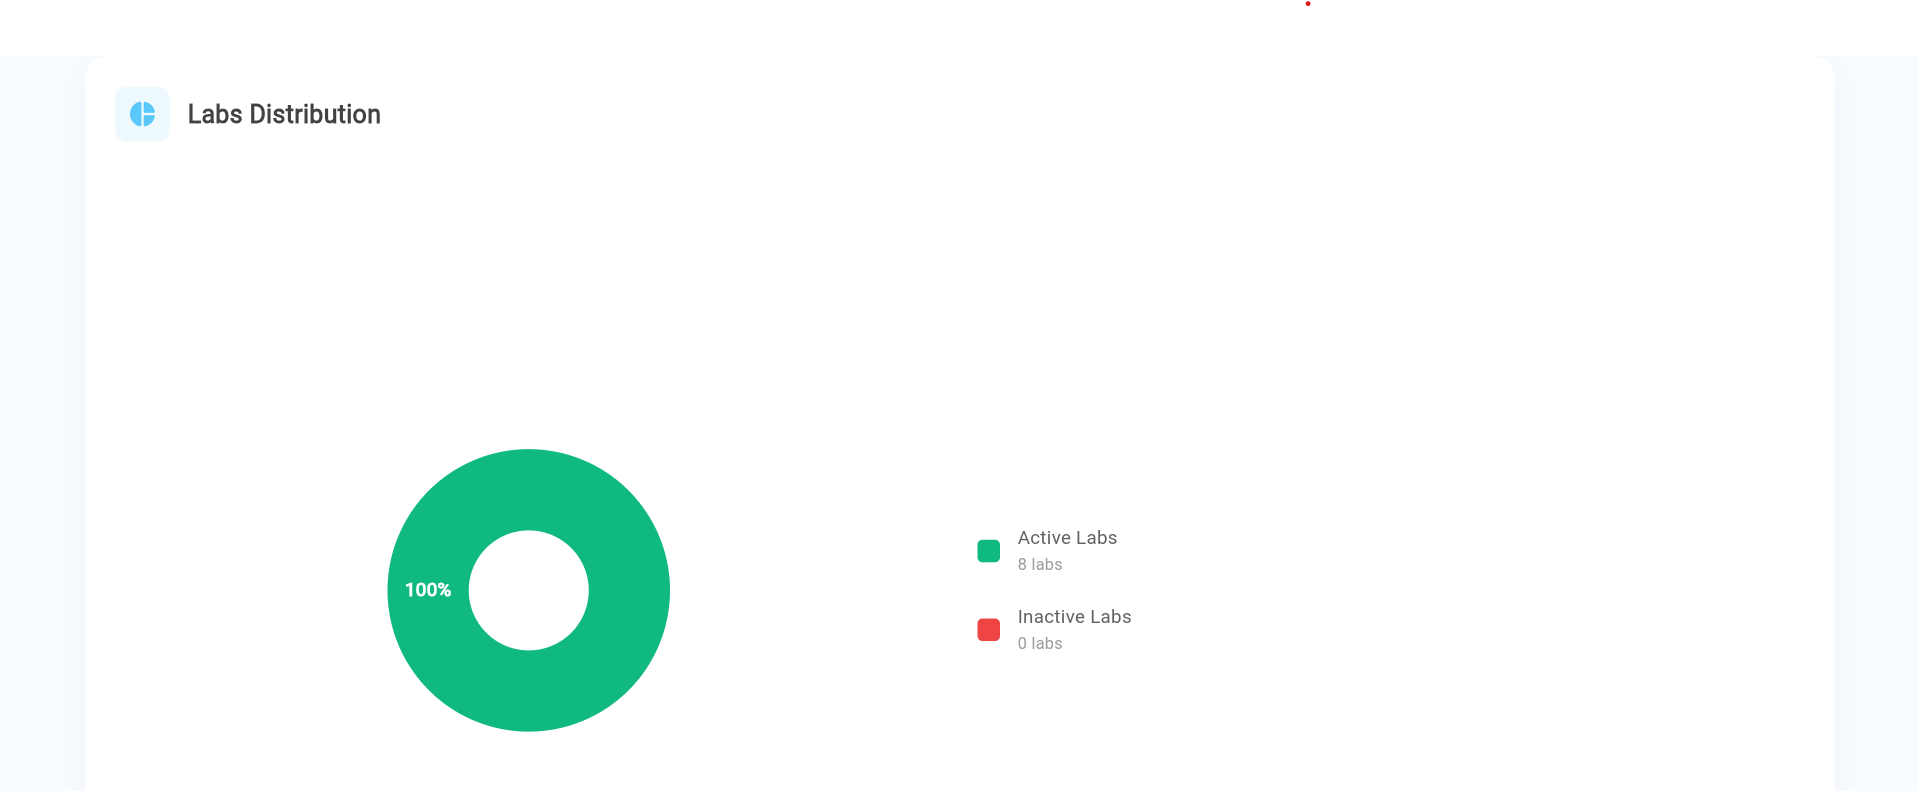
\includegraphics[width=\textwidth]{images/admin_reports_labs_chart.png}
    \caption*{(b) Labs Distribution Chart}
\end{minipage}
\caption{Admin Labs Report: (a) Laboratory statistics showing total, active, and inactive labs; (b) Pie chart visualization of lab distribution by status}
\label{fig:admin_reports_labs}
\end{figure}

The labs report provides insights into laboratory registration and activity status, showing total registered labs, active versus inactive distribution, and overall platform health indicators through the active rate percentage.

\textbf{Subscription Analytics:}
\begin{figure}[H]
\centering
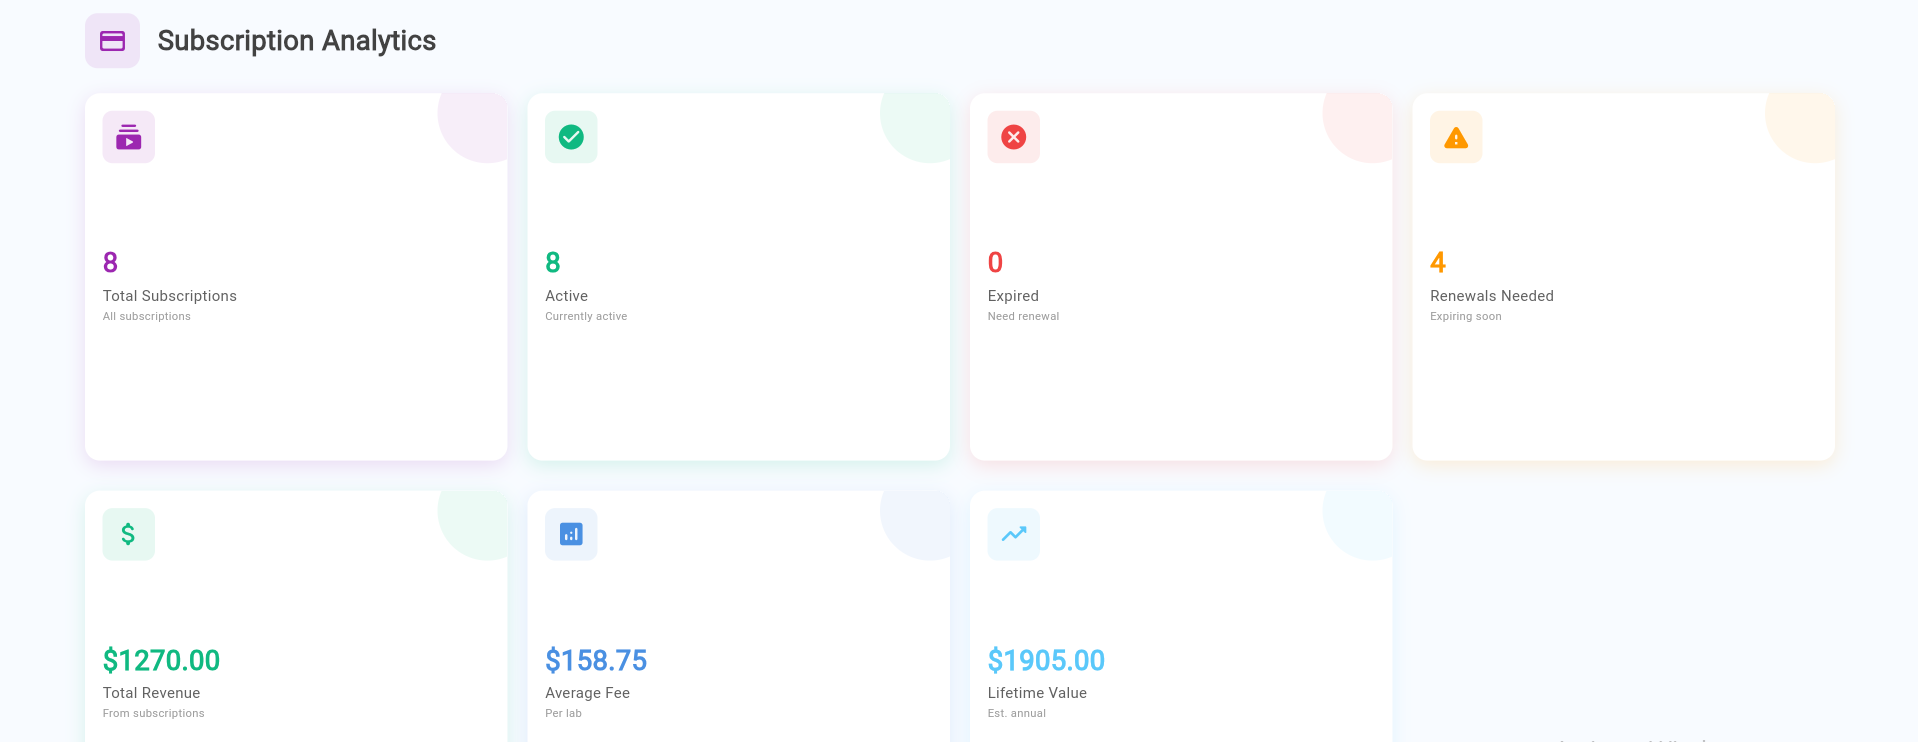
\includegraphics[width=0.7\textwidth]{images/admin_reports_subscriptions.png}
\caption{Admin Subscription Analytics Report}
\label{fig:admin_reports_subscriptions}
\end{figure}

The subscription analytics report tracks subscription lifecycle metrics including total subscriptions, active and expired counts, renewals needed, total revenue generated, average subscription fee, and estimated lifetime value per customer. This helps administrators monitor subscription health and plan for revenue forecasting.

\subsubsection{Owner Dashboard}
Laboratory owners receive comprehensive lab performance insights and management tools for their specific laboratory operations.

\begin{figure}[H]
\centering
\includegraphics[width=0.8\textwidth]{images/owner_sidebar.png}
\caption{Owner Dashboard Sidebar Navigation}
\label{fig:owner_sidebar}
\end{figure}

\textbf{Available Tabs:}

\textbf{1. Dashboard Overview}
\begin{figure}[H]
\centering
\includegraphics[width=0.9\textwidth]{images/owner_dashboard_overview.png}
\caption{Owner Dashboard Overview Tab}
\label{fig:owner_overview}
\end{figure}
Performance overview showing total orders (today/week/month), pending results, completed tests, and revenue summaries with visual charts and KPIs.

\textbf{2. Staff Management}
\begin{figure}[H]
\centering
\includegraphics[width=0.9\textwidth]{images/owner_staff.png}
\caption{Owner Staff Management Tab}
\label{fig:owner_staff}
\end{figure}
Individual staff member performance tracking with orders processed, results entered, and samples collected. Includes staff scheduling and productivity metrics.

\textbf{3. Inventory Management}
\begin{figure}[H]
\centering
\includegraphics[width=0.9\textwidth]{images/owner_inventory.png}
\caption{Owner Inventory Management Tab}
\label{fig:owner_inventory}
\end{figure}
Low stock alerts, inventory turnover rates, and reorder recommendations based on usage patterns. Tracks reagent and consumable levels across all devices.

\textbf{4. Financial Reports}
\begin{figure}[H]
\centering
\includegraphics[width=0.9\textwidth]{images/owner_financial.png}
\caption{Owner Financial Reports Tab}
\label{fig:owner_financial}
\end{figure}
Revenue by test type, payment collection rates, outstanding invoices, and profit margins. Includes detailed financial statements and export capabilities.

\textbf{5. Audit Logs}
\begin{figure}[H]
\centering
\includegraphics[width=0.9\textwidth]{images/owner_audit.png}
\caption{Owner Audit Logs Tab}
\label{fig:owner_audit}
\end{figure}
Comprehensive tracking of all staff activities including login times, patient creation, order processing, result entry, sample collection, and inventory management.

\subsubsection{Doctor Dashboard}
Physicians access patient-focused views through a streamlined single-page interface optimized for reviewing test results and managing patient orders.

\begin{figure}[H]
\centering
\includegraphics[width=0.9\textwidth]{images/doctor_dashboard_main.png}
\caption{Doctor Dashboard Main Interface}
\label{fig:doctor_main}
\end{figure}

The doctor dashboard features an AppBar navigation with notification access, profile management, and logout functionality. The main interface displays a searchable list of patient orders with test results.

\textbf{Key Features:}

\textbf{1. Patient Search and Order List}
\begin{figure}[H]
\centering
\includegraphics[width=0.9\textwidth]{images/doctor_patients_list.png}
\caption{Doctor Patient Search and Order List}
\label{fig:doctor_patients_list}
\end{figure}
Real-time search functionality allows doctors to quickly find patients by name or order ID. The interface displays a comprehensive list of patient orders with expandable cards showing order details, test status, and result availability.

\textbf{2. Test Result Viewing}
\begin{figure}[H]
\centering
\includegraphics[width=0.9\textwidth]{images/doctor_results_view.png}
\caption{Doctor Test Results View}
\label{fig:doctor_results_view}
\end{figure}
Detailed test results are displayed with reference ranges, abnormal value highlighting, and PDF download capabilities for comprehensive patient reports.

\subsubsection{Staff Dashboard}
Laboratory staff receive task-oriented workflows for efficient operations with prioritized work queues and streamlined data entry interfaces.

\begin{figure}[H]
\centering
\includegraphics[width=0.8\textwidth]{images/staff_sidebar.png}
\caption{Staff Dashboard Sidebar Navigation}
\label{fig:staff_sidebar}
\end{figure}

\textbf{Available Tabs:}

\textbf{1. Dashboard Overview}
\begin{figure}[H]
\centering
\includegraphics[width=0.9\textwidth]{images/staff_dashboard_overview.png}
\caption{Staff Dashboard Overview Tab}
\label{fig:staff_overview}
\end{figure}
Personal work queue with prioritized tasks including samples to collect, results to enter, and orders to process. Shows daily productivity metrics.

\textbf{2. Sample Collection}
\begin{figure}[H]
\centering
\includegraphics[width=0.9\textwidth]{images/staff_collection.png}
\caption{Staff Sample Collection Tab}
\label{fig:staff_collection}
\end{figure}
Barcode scanning interface with patient verification, sample labeling, and collection timestamp recording. Includes collection status updates.

\textbf{3. Result Entry}
\begin{figure}[H]
\centering
\includegraphics[width=0.9\textwidth]{images/staff_results.png}
\caption{Staff Result Entry Tab}
\label{fig:staff_results}
\end{figure}
Streamlined data entry forms with validation rules, normal range indicators, and quality control flags. Supports both manual entry and HL7 import.

\textbf{4. Upload Results}
\begin{figure}[H]
\centering
\includegraphics[width=0.9\textwidth]{images/staff_upload.png}
\caption{Staff Upload Results Tab}
\label{fig:staff_upload}
\end{figure}
Interface for uploading test results with file validation, batch processing, and result verification workflows.

\textbf{5. Inventory}
\begin{figure}[H]
\centering
\includegraphics[width=0.9\textwidth]{images/staff_inventory.png}
\caption{Staff Inventory Tab}
\label{fig:staff_inventory}
\end{figure}
Real-time inventory tracking with low stock alerts and reorder request capabilities for laboratory consumables and reagents.

\subsubsection{Patient Dashboard}
Patients access their personal health information through an intuitive, mobile-friendly interface designed for easy navigation and quick access to test results.

\begin{figure}[H]
\centering
\includegraphics[width=0.9\textwidth]{images/patient_dashboard_main.png}
\caption{Patient Dashboard Main Interface}
\label{fig:patient_main}
\end{figure}

The patient dashboard uses AppBar navigation with notification badges, profile access, and logout functionality. The main interface displays a chronological list of test orders with status indicators.

\textbf{Key Features:}

\textbf{1. Order Status Overview}
\begin{figure}[H]
\centering
\includegraphics[width=0.9\textwidth]{images/patient_orders_list.png}
\caption{Patient Orders List View}
\label{fig:patient_orders_list}
\end{figure}
Comprehensive list of all test orders showing current status, order dates, and completion progress. Each order card displays key information at a glance.

\textbf{2. Test Result Access}
\begin{figure}[H]
\centering
\includegraphics[width=0.9\textwidth]{images/patient_result_details.png}
\caption{Patient Test Result Details}
\label{fig:patient_result_details}
\end{figure}
Detailed test results with reference ranges, clinical interpretations, and downloadable PDF reports. Results are color-coded for normal/abnormal values.

\textbf{3. Notification Management}
\begin{figure}[H]
\centering
\includegraphics[width=0.9\textwidth]{images/patient_notifications.png}
\caption{Patient Notifications Dialog}
\label{fig:patient_notifications}
\end{figure}
Centralized notification center showing WhatsApp, SMS, and email alerts with read/unread status. Includes direct access to related orders and results.

\textbf{4. Profile and Settings}
\begin{figure}[H]
\centering
\includegraphics[width=0.9\textwidth]{images/patient_profile.png}
\caption{Patient Profile Management}
\label{fig:patient_profile}
\end{figure}
Personal information management including contact details, emergency contacts, and communication preferences. Allows updating account settings and notification preferences.

\subsection{Notification System}

The system implements multi-channel notifications via WhatsApp, SMS, email, and in-app alerts. Notifications cover order status updates, result availability, invoice generation with automatic PDF delivery, inventory alerts, and system events. Invoice PDFs are automatically sent to patients via WhatsApp and email immediately after order creation, ensuring prompt receipt delivery.

\subsection{Invoice Management}

The system provides comprehensive invoice generation and payment tracking for laboratory services. When an order is created, payment is applied and recorded manually by staff members. Lab owners and administrative staff can record payment information (cash, check, bank transfer), track payment status, and generate receipt PDFs. The system automatically sends invoice PDFs to patients via WhatsApp and email immediately after order creation, ensuring patients receive their receipts promptly. The invoice module maintains a complete financial history with audit trails for accounting purposes.

\subsection{Public Marketing Pages}

The public website includes a responsive landing page with featured services, searchable test catalog, testimonials section, lab locations, and contact forms. The site is optimized for mobile devices with clear calls-to-action. A comprehensive lab finder feature allows users to discover accredited medical laboratories in their area, view detailed lab information including available tests, operating hours, and contact details. Users can search labs by name or location, compare services, and contact labs directly via phone or email. Patients can browse available tests and pricing online, but orders are created manually by lab staff during patient visits to the facility.

\section{User Acceptance Testing}

Usability testing with 15 participants (3 per role) showed positive results across all user types. Participants completed predefined workflow scenarios with high success rates and reported the system as intuitive and efficient.

\textbf{Key Feedback:}
\begin{itemize}
    \item HL7 automation significantly reduces manual work
    \item WhatsApp notifications well-received by patients
    \item Dashboards provide clear overview of relevant information
    \item Suggestions included bulk result entry, trend analysis, and enhanced financial reporting
\end{itemize}

\section{Summary}

The Medical Lab System successfully implements all planned features. Key achievements include:

\begin{itemize}
    \item \textbf{Automated HL7 integration} eliminates manual result entry
    \item \textbf{Multi-channel notifications} via WhatsApp, SMS, and email
    \item \textbf{Role-specific dashboards} for efficient workflow management
    \item \textbf{Comprehensive audit logging} tracks all staff activities for accountability and monitoring    \item \textbf{Enhanced lab finder} allows patients to discover and compare local laboratories with detailed test information    \item \textbf{Automatic invoice PDF delivery} ensures patients receive receipts immediately
    \item \textbf{Enhanced patient profile management} with complete personal information updates
    \item \textbf{Invoice management and payment tracking} for financial operations
    \item \textbf{Positive user feedback} with intuitive interface design
    \item \textbf{Cross-platform support} via Flutter framework
\end{itemize}

The system demonstrates good performance, security, and usability for medical laboratory operations.

% Chapter 5: Discussion
\chapter{Discussion}
\section{Design Effectiveness}
The technology stack (Node.js, MongoDB, Flutter) enabled rapid development and cross-platform deployment. Role-specific dashboards improve workflow efficiency, while HL7 integration automates result import, reducing manual data entry significantly.

\section{Comparison with Existing Systems}
This system provides a cost-effective alternative to commercial LIMS while incorporating modern features like WhatsApp notifications and mobile access. Compared to open-source alternatives \cite{miso-lims, iskylims, metalims}, it focuses on general laboratory operations rather than specialized sequencing workflows.

\section{Future Enhancements}

\subsection{HL7 FHIR Migration}
While the current system uses HL7 v2.x for analyzer connectivity, migrating to HL7 FHIR (Fast Healthcare Interoperability Resources) would provide several advantages:
\begin{itemize}
    \item RESTful API architecture instead of TCP socket connections
    \item JSON-based messaging for easier integration with modern web services
    \item Better semantic interoperability with standardized resource definitions
    \item Wider compatibility with electronic health record (EHR) systems
    \item Simplified implementation for web and mobile applications
\end{itemize}

The migration would involve creating FHIR observation resources for test results, diagnostic report resources for complete lab reports, and service request resources for test orders.

\subsection{Advanced Analytics Dashboard}
The current dashboards display basic KPIs and metrics. Future versions could include:
\begin{itemize}
    \item \textbf{Trend Analysis:} Historical comparison of patient test results with graphical visualization of changes over time
    \item \textbf{Predictive Analytics:} Machine learning models to predict inventory reorder needs based on seasonal patterns and historical usage
    \item \textbf{Quality Metrics:} Track turnaround times, error rates, and staff productivity with detailed drill-down capabilities
    \item \textbf{Financial Forecasting:} Revenue projections based on historical data and seasonal trends
    \item \textbf{Custom Reports:} User-defined report builder with flexible filtering and export options
\end{itemize}

\subsection{Mobile Application Enhancements}
While Flutter provides cross-platform support, native mobile features could be enhanced:
\begin{itemize}
    \item \textbf{Push Notifications:} Native Android and iOS push notifications in addition to WhatsApp/SMS
    \item \textbf{Biometric Authentication:} Fingerprint and face recognition for secure mobile access
    \item \textbf{Offline Mode:} Local data caching for viewing past results without internet connection
    \item \textbf{Camera Integration:} Barcode scanning using device camera for faster sample collection
    \item \textbf{Geolocation:} Location-based lab finder and appointment booking
    \item \textbf{Office Hours Display:} Real-time display of laboratory operating hours and holiday schedules
\end{itemize}

\subsection{Integration Capabilities}
\begin{itemize}
    \item \textbf{National Health Systems:} Integration with Palestinian Ministry of Health systems for centralized health records
    \item \textbf{Insurance Providers:} Direct claims submission to insurance companies for automated claims processing
    \item \textbf{Hospital Information Systems:} Bidirectional data exchange with hospital HIS platforms
    \item \textbf{Telemedicine Platforms:} Integration with teleconsultation systems for remote result review
    \item \textbf{Pharmacy Systems:} Automatic prescription generation based on test results
\end{itemize}

\subsection{AI-Powered Features}
\begin{itemize}
    \item \textbf{Result Interpretation:} Natural language generation of clinical interpretations for common test panels
    \item \textbf{Anomaly Detection:} Automatic flagging of unusual result patterns that may indicate data entry errors
    \item \textbf{Voice Commands:} Voice-activated result entry for hands-free operation in the laboratory
    \item \textbf{Smart Scheduling:} AI-based appointment optimization considering staff availability and workload
\end{itemize}

\subsection{HIPAA Compliance}
To meet Health Insurance Portability and Accountability Act (HIPAA) requirements for deployment in US healthcare facilities, the following enhancements would be necessary:
\begin{itemize}
    \item \textbf{Business Associate Agreements:} Formal agreements with all third-party service providers (Twilio, MongoDB Atlas) ensuring HIPAA compliance
    \item \textbf{Encryption at Rest:} Full database encryption for all protected health information (PHI) stored in MongoDB
    \item \textbf{Encryption in Transit:} Mandatory TLS/SSL for all data transmissions including HL7 messages
    \item \textbf{Access Controls:} Enhanced role-based permissions with minimum necessary access principles; automatic session timeouts
    \item \textbf{Audit Trails:} Comprehensive logging of all PHI access, modifications, and deletions with tamper-proof storage
    \item \textbf{Breach Notification:} Automated detection and reporting system for potential security breaches
    \item \textbf{User Training:} Built-in HIPAA awareness training modules for all system users
    \item \textbf{Data Backup and Recovery:} HIPAA-compliant backup procedures with encrypted off-site storage and tested recovery plans
    \item \textbf{Patient Rights:} Features for patients to access, amend, and request restrictions on their health information
    \item \textbf{Security Risk Assessment:} Annual comprehensive security risk analysis and documentation
\end{itemize}

\section{Limitations}

\subsection{Third-Party Service Dependencies}
The system relies on external services which introduce several constraints:
\begin{itemize}
    \item \textbf{Twilio (WhatsApp/SMS):} Monthly costs scale with message volume; service disruptions affect patient notifications; rate limits apply (1 msg/second for WhatsApp)
    \item \textbf{MongoDB Atlas:} Cloud database costs increase with data volume; network latency affects query performance; depends on provider uptime
    \item \textbf{Email Service:} SMTP configuration required; potential delivery issues with spam filters; sending limits imposed by providers
\end{itemize}

Mitigation strategies include implementing fallback notification methods and caching critical data locally for improved reliability.

\subsection{Network and Infrastructure Requirements}
\begin{itemize}
    \item \textbf{Internet Connectivity:} System requires stable internet for real-time features; poor connectivity degrades user experience; offline mode not fully implemented
    \item \textbf{Bandwidth:} PDF report generation and image uploads require adequate bandwidth; slow connections affect file transfer speeds
    \item \textbf{Server Requirements:} Node.js backend requires dedicated hosting; minimum 2GB RAM and 2 CPU cores recommended for production
    \item \textbf{HL7 Network:} Analyzer devices must be on the same network or have VPN access to connect to the HL7 port (default 2575)
\end{itemize}

\subsection{Testing and Validation Constraints}
\begin{itemize}
    \item \textbf{Simulated Testing:} HL7 integration tested with simulated messages rather than actual laboratory analyzers; real-world device behavior may differ
    \item \textbf{Limited User Base:} User acceptance testing conducted with 15 participants; larger-scale testing needed to identify edge cases
    \item \textbf{Production Data:} Testing performed with synthetic data; real patient data may reveal unforeseen data quality issues
    \item \textbf{Load Testing:} Performance benchmarks based on simulated concurrent users; actual production load patterns may differ
    \item \textbf{Security Audit:} No professional penetration testing conducted; security assessment based on OWASP guidelines and automated tools
\end{itemize}
\subsection{Regulatory and Compliance}
\begin{itemize}
    \item \textbf{Medical Device Regulations:} System not certified as medical device software; regulatory approval required for clinical use in many jurisdictions
    \item \textbf{Data Protection:} GDPR compliance considerations needed for European deployment; local Palestinian data protection laws need verification
    \item \textbf{Clinical Validation:} Test result ranges and normal values require validation by qualified medical professionals
    \item \textbf{Healthcare Standards:} Compliance with regional healthcare standards and certification requirements not yet obtained
\end{itemize}

\subsection{Technical Limitations}
\begin{itemize}
    \item \textbf{HL7 v2.x Format:} Older standard with limited semantic clarity; requires custom mapping for each analyzer type; less flexible than modern alternatives
    \item \textbf{Single Database:} MongoDB as single data store; no redundancy or failover configured; backup strategy relies on MongoDB Atlas automated backups
    \item \textbf{Scalability:} Current architecture suitable for small-to-medium labs; high-volume facilities may require microservices architecture and load balancing
    \item \textbf{Localization:} User interface in English only; Arabic language support would require right-to-left (RTL) layout implementation and translation
    \item \textbf{Browser Compatibility:} Web frontend optimized for modern browsers; limited testing on older browsers and Internet Explorer
\end{itemize}

\subsection{Functional Limitations}
\begin{itemize}
    \item \textbf{Bulk Operations:} Result entry must be done individually; no bulk import feature for multiple results
    \item \textbf{Report Customization:} PDF reports follow fixed template; labs cannot customize report layouts without code modifications
    \item \textbf{Test Catalog:} Fixed test definitions in database; adding new tests requires technical knowledge
    \item \textbf{Multi-Lab Support:} While system supports multiple labs, data isolation could be strengthened; cross-lab analytics not implemented
    \item \textbf{Audit Trail:} Logging implemented but log analysis tools not included; manual log review required for auditing
\end{itemize}

% Chapter 6: Conclusions and Recommendations
\chapter{Conclusions and Recommendations}
\section{Conclusions}
The Medical Lab System successfully delivers a functional platform for laboratory operations with automated HL7 integration, role-based dashboards, multi-channel notifications, and comprehensive invoice management. The system demonstrates the viability of modern web technologies for healthcare applications while addressing specific needs of medical laboratories.

\section{Recommendations}
\begin{itemize}
    \item Pilot deployment in real laboratory environment
    \item Extended testing with actual medical devices
    \item Security audit and compliance review
    \item Development of training materials and user documentation
    \item Exploration of FHIR standards for future interoperability
\end{itemize}

% References
\newpage
\renewcommand{\bibname}{References}
\begin{thebibliography}{99}

% Frameworks and Technologies
\bibitem{flutter}
Google LLC, ``Flutter: Build apps for any screen,'' Flutter Documentation, 2024. [Online]. Available: \url{https://flutter.dev}

\bibitem{dart}
Google LLC, ``Dart Programming Language,'' Dart Documentation, 2024. [Online]. Available: \url{https://dart.dev}

\bibitem{express}
StrongLoop, IBM, and other expressjs.com contributors, ``Express.js: Fast, unopinionated, minimalist web framework for Node.js,'' 2024. [Online]. Available: \url{https://expressjs.com}

\bibitem{nodejs}
OpenJS Foundation, ``Node.js: JavaScript runtime built on Chrome's V8 JavaScript engine,'' 2024. [Online]. Available: \url{https://nodejs.org}

\bibitem{mongodb}
MongoDB Inc., ``MongoDB Documentation: The Developer Data Platform,'' 2024. [Online]. Available: \url{https://www.mongodb.com/docs}

\bibitem{mongoose}
Automattic Inc., ``Mongoose: Elegant MongoDB object modeling for Node.js,'' 2024. [Online]. Available: \url{https://mongoosejs.com}

% HL7 Standards
\bibitem{hl7}
HL7 International, ``HL7 Version 2 Product Brief,'' 2024. [Online]. Available: \url{https://www.hl7.org/implement/standards/product_brief.cfm?product_id=185}

\bibitem{hl7-fhir}
HL7 International, ``FHIR (Fast Healthcare Interoperability Resources) Specification,'' 2024. [Online]. Available: \url{https://www.hl7.org/fhir/}

\bibitem{hl7-messaging}
R. H. Dolin et al., ``HL7 Clinical Document Architecture, Release 2,'' \textit{Journal of the American Medical Informatics Association}, vol. 13, no. 1, pp. 30--39, 2006.

% Communication APIs
\bibitem{twilio}
Twilio Inc., ``Twilio: Communication APIs for SMS, Voice, Video, and Authentication,'' 2024. [Online]. Available: \url{https://www.twilio.com/docs}

\bibitem{firebase}
Google LLC, ``Firebase Cloud Messaging: Cross-platform messaging solution,'' Firebase Documentation, 2024. [Online]. Available: \url{https://firebase.google.com/docs/cloud-messaging}

\bibitem{nodemailer}
Andris Reinman, ``Nodemailer: Send emails from Node.js,'' 2024. [Online]. Available: \url{https://nodemailer.com}

% Security
\bibitem{jwt}
Internet Engineering Task Force, ``RFC 7519: JSON Web Token (JWT),'' 2015. [Online]. Available: \url{https://tools.ietf.org/html/rfc7519}

\bibitem{bcrypt}
N. Provos and D. Mazières, ``A Future-Adaptable Password Scheme,'' in \textit{Proceedings of the USENIX Annual Technical Conference}, 1999, pp. 81--91.

\bibitem{owasp}
OWASP Foundation, ``OWASP Top Ten Web Application Security Risks,'' 2021. [Online]. Available: \url{https://owasp.org/www-project-top-ten/}

% LIMS Academic References
\bibitem{miso-lims}
MISO LIMS Development Team, ``MISO: An open-source LIMS for NGS sequencing centres,'' GitHub repository, 2024. [Online]. Available: \url{https://github.com/miso-lims/miso-lims}

\bibitem{iskylims}
BU-ISCIII Team, ``iSkyLIMS: An open-source LIMS for Next Generation Sequencing sample management,'' GitHub repository, 2024. [Online]. Available: \url{https://github.com/BU-ISCIII/iskylims}

\bibitem{metalims}
C. Heinle et al., ``MetaLIMS, a simple open-source laboratory information management system for small metagenomic labs,'' \textit{GigaScience}, vol. 6, no. 6, pp. 1--8, Jun. 2017.

\bibitem{labware}
LabWare Inc., ``LabWare LIMS: Laboratory Information Management System,'' 2024. [Online]. Available: \url{https://www.labware.com}

% HL7 Integration Studies
\bibitem{alani-hl7-notif}
A. Al-Ani et al., ``HL7 Middleware Framework for Laboratory Notifications for Notifiable Diseases,'' \textit{Studies in Health Technology and Informatics}, vol. 214, pp. 1--7, 2015.

\bibitem{alani-hl7-early}
A. Al-Ani et al., ``Medical data integration using HL7 standards for patient's early identification,'' \textit{PLoS ONE}, vol. 16, no. 12, e0262067, 2021.

% Healthcare IT and LIMS Research
\bibitem{digital-health}
E. Coiera, ``Guide to Health Informatics,'' 3rd ed. Boca Raton, FL, USA: CRC Press, 2015.

\bibitem{ehrs}
D. F. Sittig and H. Singh, ``A new sociotechnical model for studying health information technology in complex adaptive healthcare systems,'' \textit{Quality and Safety in Health Care}, vol. 19, no. Suppl 3, pp. i68--i74, 2010.

% Software Engineering
\bibitem{agile}
K. Beck et al., ``Manifesto for Agile Software Development,'' 2001. [Online]. Available: \url{https://agilemanifesto.org}

\bibitem{rest}
R. T. Fielding, ``Architectural Styles and the Design of Network-based Software Architectures,'' Ph.D. dissertation, University of California, Irvine, 2000.

\bibitem{nosql}
P. J. Sadalage and M. Fowler, \textit{NoSQL Distilled: A Brief Guide to the Emerging World of Polyglot Persistence}. Upper Saddle River, NJ, USA: Addison-Wesley, 2012.

% Mobile Development
\bibitem{cross-platform}
A. Biørn-Hansen et al., ``An Empirical Study of Cross-Platform Mobile Development in Industry,'' \textit{Wireless Communications and Mobile Computing}, vol. 2018, pp. 1--12, 2018.

\bibitem{flutter-arch}
M. Nicola and G. Scanniello, ``Flutter: A Cross-Platform Framework for Mobile Application Development,'' in \textit{Proceedings of the International Conference on Mobile Software Engineering and Systems}, 2022, pp. 142--146.

\end{thebibliography}

% Appendices
\appendix
\chapter{Project Disclaimer}
This report was prepared by the student of the Computer Engineering Department, Faculty of Engineering, An-Najah National University, as part of graduation project requirements. The views, conclusions, and recommendations are those of the student author only. The University and Department accept no responsibility for any use made of this report beyond its original academic purpose.

\chapter{Citation Style}
All references follow the IEEE citation style.

\end{document}
